\documentclass[twoside]{book}

% Packages required by doxygen
\usepackage{fixltx2e}
\usepackage{calc}
\usepackage{doxygen}
\usepackage[export]{adjustbox} % also loads graphicx
\usepackage{graphicx}
\usepackage[utf8]{inputenc}
\usepackage{makeidx}
\usepackage{multicol}
\usepackage{multirow}
\PassOptionsToPackage{warn}{textcomp}
\usepackage{textcomp}
\usepackage[nointegrals]{wasysym}
\usepackage[table]{xcolor}

% Font selection
\usepackage[T1]{fontenc}
\usepackage[scaled=.90]{helvet}
\usepackage{courier}
\usepackage{amssymb}
\usepackage{sectsty}
\renewcommand{\familydefault}{\sfdefault}
\allsectionsfont{%
  \fontseries{bc}\selectfont%
  \color{darkgray}%
}
\renewcommand{\DoxyLabelFont}{%
  \fontseries{bc}\selectfont%
  \color{darkgray}%
}
\newcommand{\+}{\discretionary{\mbox{\scriptsize$\hookleftarrow$}}{}{}}

% Page & text layout
\usepackage{geometry}
\geometry{%
  a4paper,%
  top=2.5cm,%
  bottom=2.5cm,%
  left=2.5cm,%
  right=2.5cm%
}
\tolerance=750
\hfuzz=15pt
\hbadness=750
\setlength{\emergencystretch}{15pt}
\setlength{\parindent}{0cm}
\setlength{\parskip}{3ex plus 2ex minus 2ex}
\makeatletter
\renewcommand{\paragraph}{%
  \@startsection{paragraph}{4}{0ex}{-1.0ex}{1.0ex}{%
    \normalfont\normalsize\bfseries\SS@parafont%
  }%
}
\renewcommand{\subparagraph}{%
  \@startsection{subparagraph}{5}{0ex}{-1.0ex}{1.0ex}{%
    \normalfont\normalsize\bfseries\SS@subparafont%
  }%
}
\makeatother

% Headers & footers
\usepackage{fancyhdr}
\pagestyle{fancyplain}
\fancyhead[LE]{\fancyplain{}{\bfseries\thepage}}
\fancyhead[CE]{\fancyplain{}{}}
\fancyhead[RE]{\fancyplain{}{\bfseries\leftmark}}
\fancyhead[LO]{\fancyplain{}{\bfseries\rightmark}}
\fancyhead[CO]{\fancyplain{}{}}
\fancyhead[RO]{\fancyplain{}{\bfseries\thepage}}
\fancyfoot[LE]{\fancyplain{}{}}
\fancyfoot[CE]{\fancyplain{}{}}
\fancyfoot[RE]{\fancyplain{}{\bfseries\scriptsize Generated by Doxygen }}
\fancyfoot[LO]{\fancyplain{}{\bfseries\scriptsize Generated by Doxygen }}
\fancyfoot[CO]{\fancyplain{}{}}
\fancyfoot[RO]{\fancyplain{}{}}
\renewcommand{\footrulewidth}{0.4pt}
\renewcommand{\chaptermark}[1]{%
  \markboth{#1}{}%
}
\renewcommand{\sectionmark}[1]{%
  \markright{\thesection\ #1}%
}

% Indices & bibliography
\usepackage{natbib}
\usepackage[titles]{tocloft}
\setcounter{tocdepth}{3}
\setcounter{secnumdepth}{5}
\makeindex

% Hyperlinks (required, but should be loaded last)
\usepackage{ifpdf}
\ifpdf
  \usepackage[pdftex,pagebackref=true]{hyperref}
\else
  \usepackage[ps2pdf,pagebackref=true]{hyperref}
\fi
\hypersetup{%
  colorlinks=true,%
  linkcolor=blue,%
  citecolor=blue,%
  unicode%
}

% Custom commands
\newcommand{\clearemptydoublepage}{%
  \newpage{\pagestyle{empty}\cleardoublepage}%
}

\usepackage{caption}
\captionsetup{labelsep=space,justification=centering,font={bf},singlelinecheck=off,skip=4pt,position=top}

%===== C O N T E N T S =====

\begin{document}

% Titlepage & ToC
\hypersetup{pageanchor=false,
             bookmarksnumbered=true,
             pdfencoding=unicode
            }
\pagenumbering{roman}
\begin{titlepage}
\vspace*{7cm}
\begin{center}%
{\Large C\+U\+D\+A\+Prob3++ }\\
\vspace*{1cm}
{\large Generated by Doxygen 1.8.11}\\
\end{center}
\end{titlepage}
\clearemptydoublepage
\tableofcontents
\clearemptydoublepage
\pagenumbering{arabic}
\hypersetup{pageanchor=true}

%--- Begin generated contents ---
\chapter{Hierarchical Index}
\section{Class Hierarchy}
This inheritance list is sorted roughly, but not completely, alphabetically\+:\begin{DoxyCompactList}
\item \contentsline{section}{cudaprob3\+:\+:Propagator$<$ F\+L\+O\+A\+T\+\_\+T $>$}{\pageref{classcudaprob3_1_1Propagator}}{}
\begin{DoxyCompactList}
\item \contentsline{section}{cudaprob3\+:\+:Cpu\+Propagator$<$ F\+L\+O\+A\+T\+\_\+T $>$}{\pageref{classcudaprob3_1_1CpuPropagator}}{}
\item \contentsline{section}{cudaprob3\+:\+:Cuda\+Propagator$<$ F\+L\+O\+A\+T\+\_\+T $>$}{\pageref{classcudaprob3_1_1CudaPropagator}}{}
\item \contentsline{section}{cudaprob3\+:\+:Cuda\+Propagator\+Single$<$ F\+L\+O\+A\+T\+\_\+T $>$}{\pageref{classcudaprob3_1_1CudaPropagatorSingle}}{}
\end{DoxyCompactList}
\end{DoxyCompactList}

\chapter{Class Index}
\section{Class List}
Here are the classes, structs, unions and interfaces with brief descriptions\+:\begin{DoxyCompactList}
\item\contentsline{section}{\hyperlink{classcudaprob3_1_1CpuPropagator}{cudaprob3\+::\+Cpu\+Propagator$<$ F\+L\+O\+A\+T\+\_\+\+T $>$} \\*Multi-\/threaded C\+PU neutrino propagation. Derived from \hyperlink{classcudaprob3_1_1Propagator}{Propagator} }{\pageref{classcudaprob3_1_1CpuPropagator}}{}
\item\contentsline{section}{\hyperlink{classcudaprob3_1_1CudaPropagator}{cudaprob3\+::\+Cuda\+Propagator$<$ F\+L\+O\+A\+T\+\_\+\+T $>$} \\*Multi-\/\+G\+PU neutrino propagation. Derived from \hyperlink{classcudaprob3_1_1Propagator}{Propagator} }{\pageref{classcudaprob3_1_1CudaPropagator}}{}
\item\contentsline{section}{\hyperlink{classcudaprob3_1_1CudaPropagatorSingle}{cudaprob3\+::\+Cuda\+Propagator\+Single$<$ F\+L\+O\+A\+T\+\_\+\+T $>$} \\*Single-\/\+G\+PU neutrino propagation. Derived from \hyperlink{classcudaprob3_1_1Propagator}{Propagator} }{\pageref{classcudaprob3_1_1CudaPropagatorSingle}}{}
\item\contentsline{section}{\hyperlink{classcudaprob3_1_1Propagator}{cudaprob3\+::\+Propagator$<$ F\+L\+O\+A\+T\+\_\+\+T $>$} \\*Abstract base class of the library which sets up input parameter on the host. Concrete implementation of calcuations is provided in derived classes }{\pageref{classcudaprob3_1_1Propagator}}{}
\end{DoxyCompactList}

\chapter{Class Documentation}
\hypertarget{classcudaprob3_1_1CpuPropagator}{}\section{cudaprob3\+:\+:Cpu\+Propagator$<$ F\+L\+O\+A\+T\+\_\+T $>$ Class Template Reference}
\label{classcudaprob3_1_1CpuPropagator}\index{cudaprob3\+::\+Cpu\+Propagator$<$ F\+L\+O\+A\+T\+\_\+\+T $>$@{cudaprob3\+::\+Cpu\+Propagator$<$ F\+L\+O\+A\+T\+\_\+\+T $>$}}


Multi-\/threaded C\+PU neutrino propagation. Derived from \hyperlink{classcudaprob3_1_1Propagator}{Propagator}.  




Inheritance diagram for cudaprob3\+:\+:Cpu\+Propagator$<$ F\+L\+O\+A\+T\+\_\+T $>$\+:\nopagebreak
\begin{figure}[H]
\begin{center}
\leavevmode
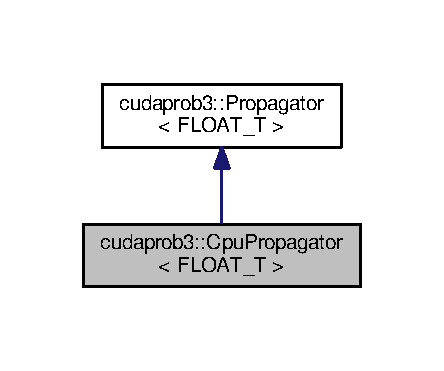
\includegraphics[width=213pt]{classcudaprob3_1_1CpuPropagator__inherit__graph}
\end{center}
\end{figure}


Collaboration diagram for cudaprob3\+:\+:Cpu\+Propagator$<$ F\+L\+O\+A\+T\+\_\+T $>$\+:\nopagebreak
\begin{figure}[H]
\begin{center}
\leavevmode
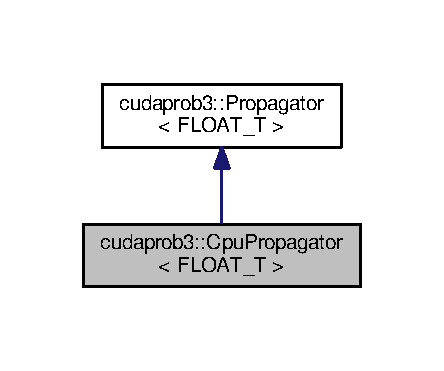
\includegraphics[width=213pt]{classcudaprob3_1_1CpuPropagator__coll__graph}
\end{center}
\end{figure}
\subsection*{Public Member Functions}
\begin{DoxyCompactItemize}
\item 
\hyperlink{classcudaprob3_1_1CpuPropagator_a0ba41c470627201c01d10983d785beea}{Cpu\+Propagator} (int n\+\_\+cosines, int n\+\_\+energies, int threads)
\begin{DoxyCompactList}\small\item\em Constructor. \end{DoxyCompactList}\item 
\hyperlink{classcudaprob3_1_1CpuPropagator_a344dc85d696677ffa2692b22a6bbea44}{Cpu\+Propagator} (const \hyperlink{classcudaprob3_1_1CpuPropagator}{Cpu\+Propagator} \&other)
\begin{DoxyCompactList}\small\item\em Copy constructor. \end{DoxyCompactList}\item 
\hyperlink{classcudaprob3_1_1CpuPropagator_a41038629d7e329e175e09cabbf386975}{Cpu\+Propagator} (\hyperlink{classcudaprob3_1_1CpuPropagator}{Cpu\+Propagator} \&\&other)
\begin{DoxyCompactList}\small\item\em Move constructor. \end{DoxyCompactList}\item 
\hyperlink{classcudaprob3_1_1CpuPropagator}{Cpu\+Propagator} \& \hyperlink{classcudaprob3_1_1CpuPropagator_a6b5b29810d22ca383ed9f617beec1523}{operator=} (const \hyperlink{classcudaprob3_1_1CpuPropagator}{Cpu\+Propagator} \&other)
\begin{DoxyCompactList}\small\item\em Copy assignment operator. \end{DoxyCompactList}\item 
\hyperlink{classcudaprob3_1_1CpuPropagator}{Cpu\+Propagator} \& \hyperlink{classcudaprob3_1_1CpuPropagator_ac612a070291f5cad723ce1bdbee3d602}{operator=} (\hyperlink{classcudaprob3_1_1CpuPropagator}{Cpu\+Propagator} \&\&other)
\begin{DoxyCompactList}\small\item\em Move assignment operator. \end{DoxyCompactList}\item 
void \hyperlink{classcudaprob3_1_1CpuPropagator_adfd6a6c86a5992bce66d0bcf975bc17d}{calculate\+Probabilities} (Neutrino\+Type type) override
\begin{DoxyCompactList}\small\item\em Calculate the probability of each cell. \end{DoxyCompactList}\item 
F\+L\+O\+A\+T\+\_\+T \hyperlink{classcudaprob3_1_1CpuPropagator_adb5c71e1b00dd5d436f04dfa9db0b364}{get\+Probability} (int index\+\_\+cosine, int index\+\_\+energy, Prob\+Type t) override
\begin{DoxyCompactList}\small\item\em get oscillation weight for specific cosine and energy \end{DoxyCompactList}\end{DoxyCompactItemize}


\subsection{Detailed Description}
\subsubsection*{template$<$class F\+L\+O\+A\+T\+\_\+T$>$\\*
class cudaprob3\+::\+Cpu\+Propagator$<$ F\+L\+O\+A\+T\+\_\+\+T $>$}

Multi-\/threaded C\+PU neutrino propagation. Derived from \hyperlink{classcudaprob3_1_1Propagator}{Propagator}. 


\begin{DoxyParams}{Parameters}
{\em F\+L\+O\+A\+T\+\_\+T} & The floating point type to use for calculations, i.\+e float, double \\
\hline
\end{DoxyParams}


\subsection{Constructor \& Destructor Documentation}
\index{cudaprob3\+::\+Cpu\+Propagator@{cudaprob3\+::\+Cpu\+Propagator}!Cpu\+Propagator@{Cpu\+Propagator}}
\index{Cpu\+Propagator@{Cpu\+Propagator}!cudaprob3\+::\+Cpu\+Propagator@{cudaprob3\+::\+Cpu\+Propagator}}
\subsubsection[{\texorpdfstring{Cpu\+Propagator(int n\+\_\+cosines, int n\+\_\+energies, int threads)}{CpuPropagator(int n_cosines, int n_energies, int threads)}}]{\setlength{\rightskip}{0pt plus 5cm}template$<$class F\+L\+O\+A\+T\+\_\+T $>$ {\bf cudaprob3\+::\+Cpu\+Propagator}$<$ F\+L\+O\+A\+T\+\_\+T $>$\+::{\bf Cpu\+Propagator} (
\begin{DoxyParamCaption}
\item[{int}]{n\+\_\+cosines, }
\item[{int}]{n\+\_\+energies, }
\item[{int}]{threads}
\end{DoxyParamCaption}
)\hspace{0.3cm}{\ttfamily [inline]}}\hypertarget{classcudaprob3_1_1CpuPropagator_a0ba41c470627201c01d10983d785beea}{}\label{classcudaprob3_1_1CpuPropagator_a0ba41c470627201c01d10983d785beea}


Constructor. 


\begin{DoxyParams}{Parameters}
{\em n\+\_\+cosines} & Number cosine bins \\
\hline
{\em n\+\_\+energies} & Number of energy bins \\
\hline
{\em threads} & Number of threads \\
\hline
\end{DoxyParams}
\index{cudaprob3\+::\+Cpu\+Propagator@{cudaprob3\+::\+Cpu\+Propagator}!Cpu\+Propagator@{Cpu\+Propagator}}
\index{Cpu\+Propagator@{Cpu\+Propagator}!cudaprob3\+::\+Cpu\+Propagator@{cudaprob3\+::\+Cpu\+Propagator}}
\subsubsection[{\texorpdfstring{Cpu\+Propagator(const Cpu\+Propagator \&other)}{CpuPropagator(const CpuPropagator &other)}}]{\setlength{\rightskip}{0pt plus 5cm}template$<$class F\+L\+O\+A\+T\+\_\+T $>$ {\bf cudaprob3\+::\+Cpu\+Propagator}$<$ F\+L\+O\+A\+T\+\_\+T $>$\+::{\bf Cpu\+Propagator} (
\begin{DoxyParamCaption}
\item[{const {\bf Cpu\+Propagator}$<$ F\+L\+O\+A\+T\+\_\+T $>$ \&}]{other}
\end{DoxyParamCaption}
)\hspace{0.3cm}{\ttfamily [inline]}}\hypertarget{classcudaprob3_1_1CpuPropagator_a344dc85d696677ffa2692b22a6bbea44}{}\label{classcudaprob3_1_1CpuPropagator_a344dc85d696677ffa2692b22a6bbea44}


Copy constructor. 


\begin{DoxyParams}{Parameters}
{\em other} & \\
\hline
\end{DoxyParams}
\index{cudaprob3\+::\+Cpu\+Propagator@{cudaprob3\+::\+Cpu\+Propagator}!Cpu\+Propagator@{Cpu\+Propagator}}
\index{Cpu\+Propagator@{Cpu\+Propagator}!cudaprob3\+::\+Cpu\+Propagator@{cudaprob3\+::\+Cpu\+Propagator}}
\subsubsection[{\texorpdfstring{Cpu\+Propagator(\+Cpu\+Propagator \&\&other)}{CpuPropagator(CpuPropagator &&other)}}]{\setlength{\rightskip}{0pt plus 5cm}template$<$class F\+L\+O\+A\+T\+\_\+T $>$ {\bf cudaprob3\+::\+Cpu\+Propagator}$<$ F\+L\+O\+A\+T\+\_\+T $>$\+::{\bf Cpu\+Propagator} (
\begin{DoxyParamCaption}
\item[{{\bf Cpu\+Propagator}$<$ F\+L\+O\+A\+T\+\_\+T $>$ \&\&}]{other}
\end{DoxyParamCaption}
)\hspace{0.3cm}{\ttfamily [inline]}}\hypertarget{classcudaprob3_1_1CpuPropagator_a41038629d7e329e175e09cabbf386975}{}\label{classcudaprob3_1_1CpuPropagator_a41038629d7e329e175e09cabbf386975}


Move constructor. 


\begin{DoxyParams}{Parameters}
{\em other} & \\
\hline
\end{DoxyParams}


\subsection{Member Function Documentation}
\index{cudaprob3\+::\+Cpu\+Propagator@{cudaprob3\+::\+Cpu\+Propagator}!calculate\+Probabilities@{calculate\+Probabilities}}
\index{calculate\+Probabilities@{calculate\+Probabilities}!cudaprob3\+::\+Cpu\+Propagator@{cudaprob3\+::\+Cpu\+Propagator}}
\subsubsection[{\texorpdfstring{calculate\+Probabilities(\+Neutrino\+Type type) override}{calculateProbabilities(NeutrinoType type) override}}]{\setlength{\rightskip}{0pt plus 5cm}template$<$class F\+L\+O\+A\+T\+\_\+T $>$ void {\bf cudaprob3\+::\+Cpu\+Propagator}$<$ F\+L\+O\+A\+T\+\_\+T $>$\+::calculate\+Probabilities (
\begin{DoxyParamCaption}
\item[{Neutrino\+Type}]{type}
\end{DoxyParamCaption}
)\hspace{0.3cm}{\ttfamily [inline]}, {\ttfamily [override]}, {\ttfamily [virtual]}}\hypertarget{classcudaprob3_1_1CpuPropagator_adfd6a6c86a5992bce66d0bcf975bc17d}{}\label{classcudaprob3_1_1CpuPropagator_adfd6a6c86a5992bce66d0bcf975bc17d}


Calculate the probability of each cell. 


\begin{DoxyParams}{Parameters}
{\em type} & Neutrino or Antineutrino \\
\hline
\end{DoxyParams}


Implements \hyperlink{classcudaprob3_1_1Propagator_abe3045e287c6a0646474189b3cff14c7}{cudaprob3\+::\+Propagator$<$ F\+L\+O\+A\+T\+\_\+\+T $>$}.

\index{cudaprob3\+::\+Cpu\+Propagator@{cudaprob3\+::\+Cpu\+Propagator}!get\+Probability@{get\+Probability}}
\index{get\+Probability@{get\+Probability}!cudaprob3\+::\+Cpu\+Propagator@{cudaprob3\+::\+Cpu\+Propagator}}
\subsubsection[{\texorpdfstring{get\+Probability(int index\+\_\+cosine, int index\+\_\+energy, Prob\+Type t) override}{getProbability(int index_cosine, int index_energy, ProbType t) override}}]{\setlength{\rightskip}{0pt plus 5cm}template$<$class F\+L\+O\+A\+T\+\_\+T $>$ F\+L\+O\+A\+T\+\_\+T {\bf cudaprob3\+::\+Cpu\+Propagator}$<$ F\+L\+O\+A\+T\+\_\+T $>$\+::get\+Probability (
\begin{DoxyParamCaption}
\item[{int}]{index\+\_\+cosine, }
\item[{int}]{index\+\_\+energy, }
\item[{Prob\+Type}]{t}
\end{DoxyParamCaption}
)\hspace{0.3cm}{\ttfamily [inline]}, {\ttfamily [override]}, {\ttfamily [virtual]}}\hypertarget{classcudaprob3_1_1CpuPropagator_adb5c71e1b00dd5d436f04dfa9db0b364}{}\label{classcudaprob3_1_1CpuPropagator_adb5c71e1b00dd5d436f04dfa9db0b364}


get oscillation weight for specific cosine and energy 


\begin{DoxyParams}{Parameters}
{\em index\+\_\+cosine} & Cosine bin index (zero based) \\
\hline
{\em index\+\_\+energy} & Energy bin index (zero based) \\
\hline
{\em t} & Specify which probability P(i-\/$>$j) \\
\hline
\end{DoxyParams}


Implements \hyperlink{classcudaprob3_1_1Propagator_a279ff90463e887754db8379c9582c943}{cudaprob3\+::\+Propagator$<$ F\+L\+O\+A\+T\+\_\+\+T $>$}.

\index{cudaprob3\+::\+Cpu\+Propagator@{cudaprob3\+::\+Cpu\+Propagator}!operator=@{operator=}}
\index{operator=@{operator=}!cudaprob3\+::\+Cpu\+Propagator@{cudaprob3\+::\+Cpu\+Propagator}}
\subsubsection[{\texorpdfstring{operator=(const Cpu\+Propagator \&other)}{operator=(const CpuPropagator &other)}}]{\setlength{\rightskip}{0pt plus 5cm}template$<$class F\+L\+O\+A\+T\+\_\+T $>$ {\bf Cpu\+Propagator}\& {\bf cudaprob3\+::\+Cpu\+Propagator}$<$ F\+L\+O\+A\+T\+\_\+T $>$\+::operator= (
\begin{DoxyParamCaption}
\item[{const {\bf Cpu\+Propagator}$<$ F\+L\+O\+A\+T\+\_\+T $>$ \&}]{other}
\end{DoxyParamCaption}
)\hspace{0.3cm}{\ttfamily [inline]}}\hypertarget{classcudaprob3_1_1CpuPropagator_a6b5b29810d22ca383ed9f617beec1523}{}\label{classcudaprob3_1_1CpuPropagator_a6b5b29810d22ca383ed9f617beec1523}


Copy assignment operator. 


\begin{DoxyParams}{Parameters}
{\em other} & \\
\hline
\end{DoxyParams}
\index{cudaprob3\+::\+Cpu\+Propagator@{cudaprob3\+::\+Cpu\+Propagator}!operator=@{operator=}}
\index{operator=@{operator=}!cudaprob3\+::\+Cpu\+Propagator@{cudaprob3\+::\+Cpu\+Propagator}}
\subsubsection[{\texorpdfstring{operator=(\+Cpu\+Propagator \&\&other)}{operator=(CpuPropagator &&other)}}]{\setlength{\rightskip}{0pt plus 5cm}template$<$class F\+L\+O\+A\+T\+\_\+T $>$ {\bf Cpu\+Propagator}\& {\bf cudaprob3\+::\+Cpu\+Propagator}$<$ F\+L\+O\+A\+T\+\_\+T $>$\+::operator= (
\begin{DoxyParamCaption}
\item[{{\bf Cpu\+Propagator}$<$ F\+L\+O\+A\+T\+\_\+T $>$ \&\&}]{other}
\end{DoxyParamCaption}
)\hspace{0.3cm}{\ttfamily [inline]}}\hypertarget{classcudaprob3_1_1CpuPropagator_ac612a070291f5cad723ce1bdbee3d602}{}\label{classcudaprob3_1_1CpuPropagator_ac612a070291f5cad723ce1bdbee3d602}


Move assignment operator. 


\begin{DoxyParams}{Parameters}
{\em other} & \\
\hline
\end{DoxyParams}


The documentation for this class was generated from the following file\+:\begin{DoxyCompactItemize}
\item 
cpupropagator.\+hpp\end{DoxyCompactItemize}

\hypertarget{classcudaprob3_1_1CudaPropagator}{}\section{cudaprob3\+:\+:Cuda\+Propagator$<$ F\+L\+O\+A\+T\+\_\+T $>$ Class Template Reference}
\label{classcudaprob3_1_1CudaPropagator}\index{cudaprob3\+::\+Cuda\+Propagator$<$ F\+L\+O\+A\+T\+\_\+\+T $>$@{cudaprob3\+::\+Cuda\+Propagator$<$ F\+L\+O\+A\+T\+\_\+\+T $>$}}


Multi-\/\+G\+PU neutrino propagation. Derived from \hyperlink{classcudaprob3_1_1Propagator}{Propagator}.  




Inheritance diagram for cudaprob3\+:\+:Cuda\+Propagator$<$ F\+L\+O\+A\+T\+\_\+T $>$\+:\nopagebreak
\begin{figure}[H]
\begin{center}
\leavevmode
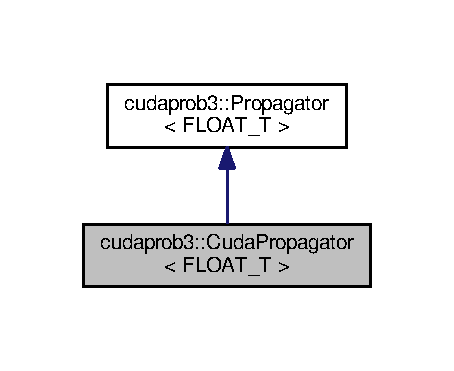
\includegraphics[width=218pt]{classcudaprob3_1_1CudaPropagator__inherit__graph}
\end{center}
\end{figure}


Collaboration diagram for cudaprob3\+:\+:Cuda\+Propagator$<$ F\+L\+O\+A\+T\+\_\+T $>$\+:\nopagebreak
\begin{figure}[H]
\begin{center}
\leavevmode
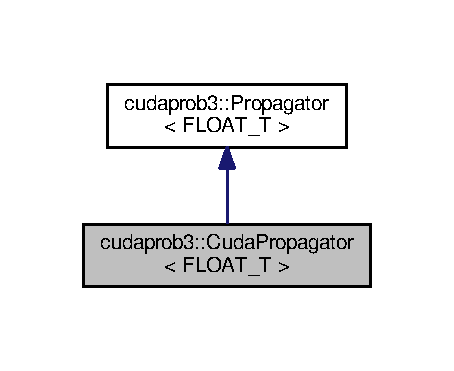
\includegraphics[width=218pt]{classcudaprob3_1_1CudaPropagator__coll__graph}
\end{center}
\end{figure}
\subsection*{Public Member Functions}
\begin{DoxyCompactItemize}
\item 
\hyperlink{classcudaprob3_1_1CudaPropagator_a9c7a73139fc4c8170357cca34c63137c}{Cuda\+Propagator} (int nc, int ne)
\begin{DoxyCompactList}\small\item\em Single G\+PU constructor for device id 0. \end{DoxyCompactList}\item 
\hyperlink{classcudaprob3_1_1CudaPropagator_abd40857d62f2b71e1926913d155382d9}{Cuda\+Propagator} (const std\+::vector$<$ int $>$ \&ids, int nc, int ne, bool fail\+On\+Invalid\+Id=true)
\begin{DoxyCompactList}\small\item\em Constructor. \end{DoxyCompactList}\item 
\hyperlink{classcudaprob3_1_1CudaPropagator_a900f5cc60675c9aeee91297bc8794095}{Cuda\+Propagator} (\hyperlink{classcudaprob3_1_1CudaPropagator}{Cuda\+Propagator} \&\&other)
\begin{DoxyCompactList}\small\item\em Move constructor. \end{DoxyCompactList}\item 
\hyperlink{classcudaprob3_1_1CudaPropagator}{Cuda\+Propagator} \& \hyperlink{classcudaprob3_1_1CudaPropagator_aa49d62a4d79bac574a53e291b084089a}{operator=} (\hyperlink{classcudaprob3_1_1CudaPropagator}{Cuda\+Propagator} \&\&other)
\begin{DoxyCompactList}\small\item\em Move assignment operator. \end{DoxyCompactList}\item 
void \hyperlink{classcudaprob3_1_1CudaPropagator_a61124bdc43a631b55ad1e9bd36a872eb}{set\+Density\+From\+File} (const std\+::string \&filename) override
\begin{DoxyCompactList}\small\item\em Set density information from file. \end{DoxyCompactList}\item 
void \hyperlink{classcudaprob3_1_1CudaPropagator_a90deddfaf8ab3c830a60d5ad5fbcfb43}{set\+Density} (const std\+::vector$<$ F\+L\+O\+A\+T\+\_\+T $>$ \&radii, const std\+::vector$<$ F\+L\+O\+A\+T\+\_\+T $>$ \&rhos) override
\begin{DoxyCompactList}\small\item\em Set density information from arrays. \end{DoxyCompactList}\item 
void \hyperlink{classcudaprob3_1_1CudaPropagator_abb9d8cc79c88f9cf6886cd334ed9e869}{set\+Neutrino\+Masses} (F\+L\+O\+A\+T\+\_\+T dm12sq, F\+L\+O\+A\+T\+\_\+T dm23sq) override
\begin{DoxyCompactList}\small\item\em Set neutrino mass differences (m\+\_\+i\+\_\+j)$^\wedge$2 in (eV)$^\wedge$2. no assumptions about mass hierarchy are made. \end{DoxyCompactList}\item 
void \hyperlink{classcudaprob3_1_1CudaPropagator_ad4fd47cd63e3b45919ae80d876698ac4}{set\+M\+N\+S\+Matrix} (F\+L\+O\+A\+T\+\_\+T theta12, F\+L\+O\+A\+T\+\_\+T theta13, F\+L\+O\+A\+T\+\_\+T theta23, F\+L\+O\+A\+T\+\_\+T d\+CP) override
\begin{DoxyCompactList}\small\item\em Set mixing angles and cp phase in radians. \end{DoxyCompactList}\item 
void \hyperlink{classcudaprob3_1_1CudaPropagator_aa2fd3a1c4c30ea967e5ac14a32ee5b7f}{set\+Energy\+List} (const std\+::vector$<$ F\+L\+O\+A\+T\+\_\+T $>$ \&list) override
\begin{DoxyCompactList}\small\item\em Set the energy bins. Energies are given in GeV. \end{DoxyCompactList}\item 
void \hyperlink{classcudaprob3_1_1CudaPropagator_afb6f73bd2451d64cfcd2b893b9b86413}{set\+Cosine\+List} (const std\+::vector$<$ F\+L\+O\+A\+T\+\_\+T $>$ \&list) override
\begin{DoxyCompactList}\small\item\em Set cosine bins. Cosines are given in radians. \end{DoxyCompactList}\item 
void \hyperlink{classcudaprob3_1_1CudaPropagator_ad639f2aa32a548b74a9a9c82d498b24a}{set\+Production\+Height} (F\+L\+O\+A\+T\+\_\+T height\+KM) override
\begin{DoxyCompactList}\small\item\em Set production height in km of neutrinos. \end{DoxyCompactList}\item 
void \hyperlink{classcudaprob3_1_1CudaPropagator_abafc49cd41569e985bd3bd9e07b31149}{calculate\+Probabilities} (Neutrino\+Type type) override
\begin{DoxyCompactList}\small\item\em Calculate the probability of each cell. \end{DoxyCompactList}\item 
F\+L\+O\+A\+T\+\_\+T \hyperlink{classcudaprob3_1_1CudaPropagator_a3cde10f1ca21db8896420649dc5d4734}{get\+Probability} (int index\+\_\+cosine, int index\+\_\+energy, Prob\+Type t) override
\begin{DoxyCompactList}\small\item\em get oscillation weight for specific cosine and energy \end{DoxyCompactList}\end{DoxyCompactItemize}


\subsection{Detailed Description}
\subsubsection*{template$<$class F\+L\+O\+A\+T\+\_\+T$>$\\*
class cudaprob3\+::\+Cuda\+Propagator$<$ F\+L\+O\+A\+T\+\_\+\+T $>$}

Multi-\/\+G\+PU neutrino propagation. Derived from \hyperlink{classcudaprob3_1_1Propagator}{Propagator}. 

This is essentially a wrapper around multiple \hyperlink{classcudaprob3_1_1CudaPropagatorSingle}{Cuda\+Propagator\+Single} instances, one per used G\+PU Most of the setters and calculation functions simply call the appropriate function for each G\+PU 
\begin{DoxyParams}{Parameters}
{\em F\+L\+O\+A\+T\+\_\+T} & The floating point type to use for calculations, i.\+e float, double \\
\hline
\end{DoxyParams}


\subsection{Constructor \& Destructor Documentation}
\index{cudaprob3\+::\+Cuda\+Propagator@{cudaprob3\+::\+Cuda\+Propagator}!Cuda\+Propagator@{Cuda\+Propagator}}
\index{Cuda\+Propagator@{Cuda\+Propagator}!cudaprob3\+::\+Cuda\+Propagator@{cudaprob3\+::\+Cuda\+Propagator}}
\subsubsection[{\texorpdfstring{Cuda\+Propagator(int nc, int ne)}{CudaPropagator(int nc, int ne)}}]{\setlength{\rightskip}{0pt plus 5cm}template$<$class F\+L\+O\+A\+T\+\_\+T $>$ {\bf cudaprob3\+::\+Cuda\+Propagator}$<$ F\+L\+O\+A\+T\+\_\+T $>$\+::{\bf Cuda\+Propagator} (
\begin{DoxyParamCaption}
\item[{int}]{nc, }
\item[{int}]{ne}
\end{DoxyParamCaption}
)\hspace{0.3cm}{\ttfamily [inline]}}\hypertarget{classcudaprob3_1_1CudaPropagator_a9c7a73139fc4c8170357cca34c63137c}{}\label{classcudaprob3_1_1CudaPropagator_a9c7a73139fc4c8170357cca34c63137c}


Single G\+PU constructor for device id 0. 


\begin{DoxyParams}{Parameters}
{\em nc} & Number cosine bins \\
\hline
{\em ne} & Number of energy bins \\
\hline
\end{DoxyParams}
\index{cudaprob3\+::\+Cuda\+Propagator@{cudaprob3\+::\+Cuda\+Propagator}!Cuda\+Propagator@{Cuda\+Propagator}}
\index{Cuda\+Propagator@{Cuda\+Propagator}!cudaprob3\+::\+Cuda\+Propagator@{cudaprob3\+::\+Cuda\+Propagator}}
\subsubsection[{\texorpdfstring{Cuda\+Propagator(const std\+::vector$<$ int $>$ \&ids, int nc, int ne, bool fail\+On\+Invalid\+Id=true)}{CudaPropagator(const std::vector< int > &ids, int nc, int ne, bool failOnInvalidId=true)}}]{\setlength{\rightskip}{0pt plus 5cm}template$<$class F\+L\+O\+A\+T\+\_\+T $>$ {\bf cudaprob3\+::\+Cuda\+Propagator}$<$ F\+L\+O\+A\+T\+\_\+T $>$\+::{\bf Cuda\+Propagator} (
\begin{DoxyParamCaption}
\item[{const std\+::vector$<$ int $>$ \&}]{ids, }
\item[{int}]{nc, }
\item[{int}]{ne, }
\item[{bool}]{fail\+On\+Invalid\+Id = {\ttfamily true}}
\end{DoxyParamCaption}
)\hspace{0.3cm}{\ttfamily [inline]}}\hypertarget{classcudaprob3_1_1CudaPropagator_abd40857d62f2b71e1926913d155382d9}{}\label{classcudaprob3_1_1CudaPropagator_abd40857d62f2b71e1926913d155382d9}


Constructor. 


\begin{DoxyParams}{Parameters}
{\em ids} & List of device ids of the G\+P\+Us to use \\
\hline
{\em nc} & Number cosine bins \\
\hline
{\em ne} & Number of energy bins \\
\hline
{\em fail\+On\+Invalid\+Id} & If true, throw exception if ids contains an invalid device id \\
\hline
\end{DoxyParams}
\index{cudaprob3\+::\+Cuda\+Propagator@{cudaprob3\+::\+Cuda\+Propagator}!Cuda\+Propagator@{Cuda\+Propagator}}
\index{Cuda\+Propagator@{Cuda\+Propagator}!cudaprob3\+::\+Cuda\+Propagator@{cudaprob3\+::\+Cuda\+Propagator}}
\subsubsection[{\texorpdfstring{Cuda\+Propagator(\+Cuda\+Propagator \&\&other)}{CudaPropagator(CudaPropagator &&other)}}]{\setlength{\rightskip}{0pt plus 5cm}template$<$class F\+L\+O\+A\+T\+\_\+T $>$ {\bf cudaprob3\+::\+Cuda\+Propagator}$<$ F\+L\+O\+A\+T\+\_\+T $>$\+::{\bf Cuda\+Propagator} (
\begin{DoxyParamCaption}
\item[{{\bf Cuda\+Propagator}$<$ F\+L\+O\+A\+T\+\_\+T $>$ \&\&}]{other}
\end{DoxyParamCaption}
)\hspace{0.3cm}{\ttfamily [inline]}}\hypertarget{classcudaprob3_1_1CudaPropagator_a900f5cc60675c9aeee91297bc8794095}{}\label{classcudaprob3_1_1CudaPropagator_a900f5cc60675c9aeee91297bc8794095}


Move constructor. 


\begin{DoxyParams}{Parameters}
{\em other} & \\
\hline
\end{DoxyParams}


\subsection{Member Function Documentation}
\index{cudaprob3\+::\+Cuda\+Propagator@{cudaprob3\+::\+Cuda\+Propagator}!calculate\+Probabilities@{calculate\+Probabilities}}
\index{calculate\+Probabilities@{calculate\+Probabilities}!cudaprob3\+::\+Cuda\+Propagator@{cudaprob3\+::\+Cuda\+Propagator}}
\subsubsection[{\texorpdfstring{calculate\+Probabilities(\+Neutrino\+Type type) override}{calculateProbabilities(NeutrinoType type) override}}]{\setlength{\rightskip}{0pt plus 5cm}template$<$class F\+L\+O\+A\+T\+\_\+T $>$ void {\bf cudaprob3\+::\+Cuda\+Propagator}$<$ F\+L\+O\+A\+T\+\_\+T $>$\+::calculate\+Probabilities (
\begin{DoxyParamCaption}
\item[{Neutrino\+Type}]{type}
\end{DoxyParamCaption}
)\hspace{0.3cm}{\ttfamily [inline]}, {\ttfamily [override]}, {\ttfamily [virtual]}}\hypertarget{classcudaprob3_1_1CudaPropagator_abafc49cd41569e985bd3bd9e07b31149}{}\label{classcudaprob3_1_1CudaPropagator_abafc49cd41569e985bd3bd9e07b31149}


Calculate the probability of each cell. 


\begin{DoxyParams}{Parameters}
{\em type} & Neutrino or Antineutrino \\
\hline
\end{DoxyParams}


Implements \hyperlink{classcudaprob3_1_1Propagator_abe3045e287c6a0646474189b3cff14c7}{cudaprob3\+::\+Propagator$<$ F\+L\+O\+A\+T\+\_\+\+T $>$}.

\index{cudaprob3\+::\+Cuda\+Propagator@{cudaprob3\+::\+Cuda\+Propagator}!get\+Probability@{get\+Probability}}
\index{get\+Probability@{get\+Probability}!cudaprob3\+::\+Cuda\+Propagator@{cudaprob3\+::\+Cuda\+Propagator}}
\subsubsection[{\texorpdfstring{get\+Probability(int index\+\_\+cosine, int index\+\_\+energy, Prob\+Type t) override}{getProbability(int index_cosine, int index_energy, ProbType t) override}}]{\setlength{\rightskip}{0pt plus 5cm}template$<$class F\+L\+O\+A\+T\+\_\+T $>$ F\+L\+O\+A\+T\+\_\+T {\bf cudaprob3\+::\+Cuda\+Propagator}$<$ F\+L\+O\+A\+T\+\_\+T $>$\+::get\+Probability (
\begin{DoxyParamCaption}
\item[{int}]{index\+\_\+cosine, }
\item[{int}]{index\+\_\+energy, }
\item[{Prob\+Type}]{t}
\end{DoxyParamCaption}
)\hspace{0.3cm}{\ttfamily [inline]}, {\ttfamily [override]}, {\ttfamily [virtual]}}\hypertarget{classcudaprob3_1_1CudaPropagator_a3cde10f1ca21db8896420649dc5d4734}{}\label{classcudaprob3_1_1CudaPropagator_a3cde10f1ca21db8896420649dc5d4734}


get oscillation weight for specific cosine and energy 


\begin{DoxyParams}{Parameters}
{\em index\+\_\+cosine} & Cosine bin index (zero based) \\
\hline
{\em index\+\_\+energy} & Energy bin index (zero based) \\
\hline
{\em t} & Specify which probability P(i-\/$>$j) \\
\hline
\end{DoxyParams}


Implements \hyperlink{classcudaprob3_1_1Propagator_a279ff90463e887754db8379c9582c943}{cudaprob3\+::\+Propagator$<$ F\+L\+O\+A\+T\+\_\+\+T $>$}.

\index{cudaprob3\+::\+Cuda\+Propagator@{cudaprob3\+::\+Cuda\+Propagator}!operator=@{operator=}}
\index{operator=@{operator=}!cudaprob3\+::\+Cuda\+Propagator@{cudaprob3\+::\+Cuda\+Propagator}}
\subsubsection[{\texorpdfstring{operator=(\+Cuda\+Propagator \&\&other)}{operator=(CudaPropagator &&other)}}]{\setlength{\rightskip}{0pt plus 5cm}template$<$class F\+L\+O\+A\+T\+\_\+T $>$ {\bf Cuda\+Propagator}\& {\bf cudaprob3\+::\+Cuda\+Propagator}$<$ F\+L\+O\+A\+T\+\_\+T $>$\+::operator= (
\begin{DoxyParamCaption}
\item[{{\bf Cuda\+Propagator}$<$ F\+L\+O\+A\+T\+\_\+T $>$ \&\&}]{other}
\end{DoxyParamCaption}
)\hspace{0.3cm}{\ttfamily [inline]}}\hypertarget{classcudaprob3_1_1CudaPropagator_aa49d62a4d79bac574a53e291b084089a}{}\label{classcudaprob3_1_1CudaPropagator_aa49d62a4d79bac574a53e291b084089a}


Move assignment operator. 


\begin{DoxyParams}{Parameters}
{\em other} & \\
\hline
\end{DoxyParams}
\index{cudaprob3\+::\+Cuda\+Propagator@{cudaprob3\+::\+Cuda\+Propagator}!set\+Cosine\+List@{set\+Cosine\+List}}
\index{set\+Cosine\+List@{set\+Cosine\+List}!cudaprob3\+::\+Cuda\+Propagator@{cudaprob3\+::\+Cuda\+Propagator}}
\subsubsection[{\texorpdfstring{set\+Cosine\+List(const std\+::vector$<$ F\+L\+O\+A\+T\+\_\+\+T $>$ \&list) override}{setCosineList(const std::vector< FLOAT_T > &list) override}}]{\setlength{\rightskip}{0pt plus 5cm}template$<$class F\+L\+O\+A\+T\+\_\+T $>$ void {\bf cudaprob3\+::\+Cuda\+Propagator}$<$ F\+L\+O\+A\+T\+\_\+T $>$\+::set\+Cosine\+List (
\begin{DoxyParamCaption}
\item[{const std\+::vector$<$ F\+L\+O\+A\+T\+\_\+T $>$ \&}]{list}
\end{DoxyParamCaption}
)\hspace{0.3cm}{\ttfamily [inline]}, {\ttfamily [override]}, {\ttfamily [virtual]}}\hypertarget{classcudaprob3_1_1CudaPropagator_afb6f73bd2451d64cfcd2b893b9b86413}{}\label{classcudaprob3_1_1CudaPropagator_afb6f73bd2451d64cfcd2b893b9b86413}


Set cosine bins. Cosines are given in radians. 


\begin{DoxyParams}{Parameters}
{\em list} & Cosine list \\
\hline
\end{DoxyParams}


Reimplemented from \hyperlink{classcudaprob3_1_1Propagator_ac2beb7d48c566ef0f07666927fbf5e3f}{cudaprob3\+::\+Propagator$<$ F\+L\+O\+A\+T\+\_\+\+T $>$}.

\index{cudaprob3\+::\+Cuda\+Propagator@{cudaprob3\+::\+Cuda\+Propagator}!set\+Density@{set\+Density}}
\index{set\+Density@{set\+Density}!cudaprob3\+::\+Cuda\+Propagator@{cudaprob3\+::\+Cuda\+Propagator}}
\subsubsection[{\texorpdfstring{set\+Density(const std\+::vector$<$ F\+L\+O\+A\+T\+\_\+\+T $>$ \&radii, const std\+::vector$<$ F\+L\+O\+A\+T\+\_\+\+T $>$ \&rhos) override}{setDensity(const std::vector< FLOAT_T > &radii, const std::vector< FLOAT_T > &rhos) override}}]{\setlength{\rightskip}{0pt plus 5cm}template$<$class F\+L\+O\+A\+T\+\_\+T $>$ void {\bf cudaprob3\+::\+Cuda\+Propagator}$<$ F\+L\+O\+A\+T\+\_\+T $>$\+::set\+Density (
\begin{DoxyParamCaption}
\item[{const std\+::vector$<$ F\+L\+O\+A\+T\+\_\+T $>$ \&}]{radii\+\_\+, }
\item[{const std\+::vector$<$ F\+L\+O\+A\+T\+\_\+T $>$ \&}]{rhos\+\_\+}
\end{DoxyParamCaption}
)\hspace{0.3cm}{\ttfamily [inline]}, {\ttfamily [override]}, {\ttfamily [virtual]}}\hypertarget{classcudaprob3_1_1CudaPropagator_a90deddfaf8ab3c830a60d5ad5fbcfb43}{}\label{classcudaprob3_1_1CudaPropagator_a90deddfaf8ab3c830a60d5ad5fbcfb43}


Set density information from arrays. 

radii\+\_\+ and rhos\+\_\+ must be same size. both radii\+\_\+ and rhos\+\_\+ must be sorted, in the same order. The density (g/cm$^\wedge$3) at a distance (km) from the center of the sphere between radii\+\_\+\mbox{[}i\mbox{]}, exclusive, and radii\+\_\+\mbox{[}j\mbox{]}, inclusive, i $<$ j is assumed to be rhos\+\_\+\mbox{[}j\mbox{]} 
\begin{DoxyParams}{Parameters}
{\em radii\+\_\+} & List of radii \\
\hline
{\em rhos\+\_\+} & List of densities \\
\hline
\end{DoxyParams}


Reimplemented from \hyperlink{classcudaprob3_1_1Propagator_a119a29681c30c9476f0b50ed07cb639d}{cudaprob3\+::\+Propagator$<$ F\+L\+O\+A\+T\+\_\+\+T $>$}.

\index{cudaprob3\+::\+Cuda\+Propagator@{cudaprob3\+::\+Cuda\+Propagator}!set\+Density\+From\+File@{set\+Density\+From\+File}}
\index{set\+Density\+From\+File@{set\+Density\+From\+File}!cudaprob3\+::\+Cuda\+Propagator@{cudaprob3\+::\+Cuda\+Propagator}}
\subsubsection[{\texorpdfstring{set\+Density\+From\+File(const std\+::string \&filename) override}{setDensityFromFile(const std::string &filename) override}}]{\setlength{\rightskip}{0pt plus 5cm}template$<$class F\+L\+O\+A\+T\+\_\+T $>$ void {\bf cudaprob3\+::\+Cuda\+Propagator}$<$ F\+L\+O\+A\+T\+\_\+T $>$\+::set\+Density\+From\+File (
\begin{DoxyParamCaption}
\item[{const std\+::string \&}]{filename}
\end{DoxyParamCaption}
)\hspace{0.3cm}{\ttfamily [inline]}, {\ttfamily [override]}, {\ttfamily [virtual]}}\hypertarget{classcudaprob3_1_1CudaPropagator_a61124bdc43a631b55ad1e9bd36a872eb}{}\label{classcudaprob3_1_1CudaPropagator_a61124bdc43a631b55ad1e9bd36a872eb}


Set density information from file. 

File must contain two columns where the first column contains the radius (km) and the second column contains the density (g/cm³). The first row must have the radius 0. The last row must have to radius of the sphere


\begin{DoxyParams}{Parameters}
{\em filename} & File with density information \\
\hline
\end{DoxyParams}


Reimplemented from \hyperlink{classcudaprob3_1_1Propagator_a7d40f7d7e0716e5b532a7a3a228d3b01}{cudaprob3\+::\+Propagator$<$ F\+L\+O\+A\+T\+\_\+\+T $>$}.

\index{cudaprob3\+::\+Cuda\+Propagator@{cudaprob3\+::\+Cuda\+Propagator}!set\+Energy\+List@{set\+Energy\+List}}
\index{set\+Energy\+List@{set\+Energy\+List}!cudaprob3\+::\+Cuda\+Propagator@{cudaprob3\+::\+Cuda\+Propagator}}
\subsubsection[{\texorpdfstring{set\+Energy\+List(const std\+::vector$<$ F\+L\+O\+A\+T\+\_\+\+T $>$ \&list) override}{setEnergyList(const std::vector< FLOAT_T > &list) override}}]{\setlength{\rightskip}{0pt plus 5cm}template$<$class F\+L\+O\+A\+T\+\_\+T $>$ void {\bf cudaprob3\+::\+Cuda\+Propagator}$<$ F\+L\+O\+A\+T\+\_\+T $>$\+::set\+Energy\+List (
\begin{DoxyParamCaption}
\item[{const std\+::vector$<$ F\+L\+O\+A\+T\+\_\+T $>$ \&}]{list}
\end{DoxyParamCaption}
)\hspace{0.3cm}{\ttfamily [inline]}, {\ttfamily [override]}, {\ttfamily [virtual]}}\hypertarget{classcudaprob3_1_1CudaPropagator_aa2fd3a1c4c30ea967e5ac14a32ee5b7f}{}\label{classcudaprob3_1_1CudaPropagator_aa2fd3a1c4c30ea967e5ac14a32ee5b7f}


Set the energy bins. Energies are given in GeV. 


\begin{DoxyParams}{Parameters}
{\em list} & Energy list \\
\hline
\end{DoxyParams}


Reimplemented from \hyperlink{classcudaprob3_1_1Propagator_a1135d977c5034e982a63c583ab4dad06}{cudaprob3\+::\+Propagator$<$ F\+L\+O\+A\+T\+\_\+\+T $>$}.

\index{cudaprob3\+::\+Cuda\+Propagator@{cudaprob3\+::\+Cuda\+Propagator}!set\+M\+N\+S\+Matrix@{set\+M\+N\+S\+Matrix}}
\index{set\+M\+N\+S\+Matrix@{set\+M\+N\+S\+Matrix}!cudaprob3\+::\+Cuda\+Propagator@{cudaprob3\+::\+Cuda\+Propagator}}
\subsubsection[{\texorpdfstring{set\+M\+N\+S\+Matrix(\+F\+L\+O\+A\+T\+\_\+\+T theta12, F\+L\+O\+A\+T\+\_\+\+T theta13, F\+L\+O\+A\+T\+\_\+\+T theta23, F\+L\+O\+A\+T\+\_\+\+T d\+C\+P) override}{setMNSMatrix(FLOAT_T theta12, FLOAT_T theta13, FLOAT_T theta23, FLOAT_T dCP) override}}]{\setlength{\rightskip}{0pt plus 5cm}template$<$class F\+L\+O\+A\+T\+\_\+T $>$ void {\bf cudaprob3\+::\+Cuda\+Propagator}$<$ F\+L\+O\+A\+T\+\_\+T $>$\+::set\+M\+N\+S\+Matrix (
\begin{DoxyParamCaption}
\item[{F\+L\+O\+A\+T\+\_\+T}]{theta12, }
\item[{F\+L\+O\+A\+T\+\_\+T}]{theta13, }
\item[{F\+L\+O\+A\+T\+\_\+T}]{theta23, }
\item[{F\+L\+O\+A\+T\+\_\+T}]{d\+CP}
\end{DoxyParamCaption}
)\hspace{0.3cm}{\ttfamily [inline]}, {\ttfamily [override]}, {\ttfamily [virtual]}}\hypertarget{classcudaprob3_1_1CudaPropagator_ad4fd47cd63e3b45919ae80d876698ac4}{}\label{classcudaprob3_1_1CudaPropagator_ad4fd47cd63e3b45919ae80d876698ac4}


Set mixing angles and cp phase in radians. 


\begin{DoxyParams}{Parameters}
{\em theta12} & \\
\hline
{\em theta13} & \\
\hline
{\em theta23} & \\
\hline
{\em d\+CP} & \\
\hline
\end{DoxyParams}


Reimplemented from \hyperlink{classcudaprob3_1_1Propagator_ad866c252d72ae6cc0ed3fc3b76c7cac7}{cudaprob3\+::\+Propagator$<$ F\+L\+O\+A\+T\+\_\+\+T $>$}.

\index{cudaprob3\+::\+Cuda\+Propagator@{cudaprob3\+::\+Cuda\+Propagator}!set\+Neutrino\+Masses@{set\+Neutrino\+Masses}}
\index{set\+Neutrino\+Masses@{set\+Neutrino\+Masses}!cudaprob3\+::\+Cuda\+Propagator@{cudaprob3\+::\+Cuda\+Propagator}}
\subsubsection[{\texorpdfstring{set\+Neutrino\+Masses(\+F\+L\+O\+A\+T\+\_\+\+T dm12sq, F\+L\+O\+A\+T\+\_\+\+T dm23sq) override}{setNeutrinoMasses(FLOAT_T dm12sq, FLOAT_T dm23sq) override}}]{\setlength{\rightskip}{0pt plus 5cm}template$<$class F\+L\+O\+A\+T\+\_\+T $>$ void {\bf cudaprob3\+::\+Cuda\+Propagator}$<$ F\+L\+O\+A\+T\+\_\+T $>$\+::set\+Neutrino\+Masses (
\begin{DoxyParamCaption}
\item[{F\+L\+O\+A\+T\+\_\+T}]{dm12sq, }
\item[{F\+L\+O\+A\+T\+\_\+T}]{dm23sq}
\end{DoxyParamCaption}
)\hspace{0.3cm}{\ttfamily [inline]}, {\ttfamily [override]}, {\ttfamily [virtual]}}\hypertarget{classcudaprob3_1_1CudaPropagator_abb9d8cc79c88f9cf6886cd334ed9e869}{}\label{classcudaprob3_1_1CudaPropagator_abb9d8cc79c88f9cf6886cd334ed9e869}


Set neutrino mass differences (m\+\_\+i\+\_\+j)$^\wedge$2 in (eV)$^\wedge$2. no assumptions about mass hierarchy are made. 


\begin{DoxyParams}{Parameters}
{\em dm12sq} & \\
\hline
{\em dm23sq} & \\
\hline
\end{DoxyParams}


Reimplemented from \hyperlink{classcudaprob3_1_1Propagator_adaa3bc796f0bca8ce177f364c559b262}{cudaprob3\+::\+Propagator$<$ F\+L\+O\+A\+T\+\_\+\+T $>$}.

\index{cudaprob3\+::\+Cuda\+Propagator@{cudaprob3\+::\+Cuda\+Propagator}!set\+Production\+Height@{set\+Production\+Height}}
\index{set\+Production\+Height@{set\+Production\+Height}!cudaprob3\+::\+Cuda\+Propagator@{cudaprob3\+::\+Cuda\+Propagator}}
\subsubsection[{\texorpdfstring{set\+Production\+Height(\+F\+L\+O\+A\+T\+\_\+\+T height\+K\+M) override}{setProductionHeight(FLOAT_T heightKM) override}}]{\setlength{\rightskip}{0pt plus 5cm}template$<$class F\+L\+O\+A\+T\+\_\+T $>$ void {\bf cudaprob3\+::\+Cuda\+Propagator}$<$ F\+L\+O\+A\+T\+\_\+T $>$\+::set\+Production\+Height (
\begin{DoxyParamCaption}
\item[{F\+L\+O\+A\+T\+\_\+T}]{height\+KM}
\end{DoxyParamCaption}
)\hspace{0.3cm}{\ttfamily [inline]}, {\ttfamily [override]}, {\ttfamily [virtual]}}\hypertarget{classcudaprob3_1_1CudaPropagator_ad639f2aa32a548b74a9a9c82d498b24a}{}\label{classcudaprob3_1_1CudaPropagator_ad639f2aa32a548b74a9a9c82d498b24a}


Set production height in km of neutrinos. 

Adds a layer of length height\+KM with zero density to the density model 
\begin{DoxyParams}{Parameters}
{\em height\+KM} & Set neutrino production height \\
\hline
\end{DoxyParams}


Reimplemented from \hyperlink{classcudaprob3_1_1Propagator_a5db866f0c9852d65cc2b1e43bbc3bef5}{cudaprob3\+::\+Propagator$<$ F\+L\+O\+A\+T\+\_\+\+T $>$}.



The documentation for this class was generated from the following file\+:\begin{DoxyCompactItemize}
\item 
cudapropagator.\+cuh\end{DoxyCompactItemize}

\hypertarget{classcudaprob3_1_1CudaPropagatorSingle}{}\section{cudaprob3\+:\+:Cuda\+Propagator\+Single$<$ F\+L\+O\+A\+T\+\_\+T $>$ Class Template Reference}
\label{classcudaprob3_1_1CudaPropagatorSingle}\index{cudaprob3\+::\+Cuda\+Propagator\+Single$<$ F\+L\+O\+A\+T\+\_\+\+T $>$@{cudaprob3\+::\+Cuda\+Propagator\+Single$<$ F\+L\+O\+A\+T\+\_\+\+T $>$}}


Single-\/\+G\+PU neutrino propagation. Derived from \hyperlink{classcudaprob3_1_1Propagator}{Propagator}.  




Inheritance diagram for cudaprob3\+:\+:Cuda\+Propagator\+Single$<$ F\+L\+O\+A\+T\+\_\+T $>$\+:\nopagebreak
\begin{figure}[H]
\begin{center}
\leavevmode
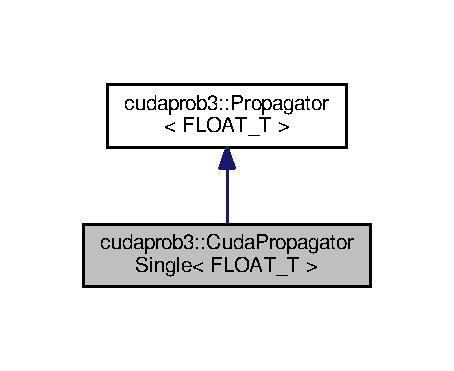
\includegraphics[width=218pt]{classcudaprob3_1_1CudaPropagatorSingle__inherit__graph}
\end{center}
\end{figure}


Collaboration diagram for cudaprob3\+:\+:Cuda\+Propagator\+Single$<$ F\+L\+O\+A\+T\+\_\+T $>$\+:\nopagebreak
\begin{figure}[H]
\begin{center}
\leavevmode
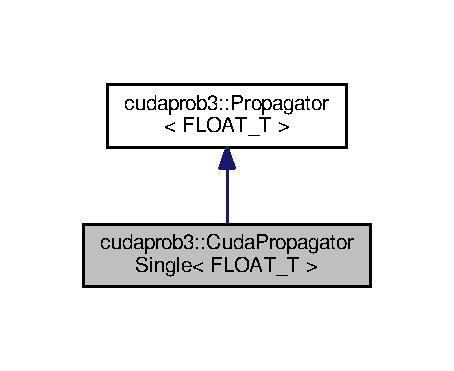
\includegraphics[width=218pt]{classcudaprob3_1_1CudaPropagatorSingle__coll__graph}
\end{center}
\end{figure}
\subsection*{Public Member Functions}
\begin{DoxyCompactItemize}
\item 
\hyperlink{classcudaprob3_1_1CudaPropagatorSingle_afdf1133d44933fee8ce26c7f7287a089}{Cuda\+Propagator\+Single} (int id, int n\+\_\+cosines\+\_\+, int n\+\_\+energies\+\_\+)
\begin{DoxyCompactList}\small\item\em Constructor. \end{DoxyCompactList}\item 
\hyperlink{classcudaprob3_1_1CudaPropagatorSingle_a367c4f257905344c3fa7ae50507e5942}{Cuda\+Propagator\+Single} (int n\+\_\+cosines, int n\+\_\+energies)
\begin{DoxyCompactList}\small\item\em Constructor which uses device id 0. \end{DoxyCompactList}\item 
\hyperlink{classcudaprob3_1_1CudaPropagatorSingle_ac779c663d73e1c2a0ac6b10d770ac0a4}{$\sim$\+Cuda\+Propagator\+Single} ()\hypertarget{classcudaprob3_1_1CudaPropagatorSingle_ac779c663d73e1c2a0ac6b10d770ac0a4}{}\label{classcudaprob3_1_1CudaPropagatorSingle_ac779c663d73e1c2a0ac6b10d770ac0a4}

\begin{DoxyCompactList}\small\item\em Destructor. \end{DoxyCompactList}\item 
\hyperlink{classcudaprob3_1_1CudaPropagatorSingle_aa97189759f1c36bc173db642529081e8}{Cuda\+Propagator\+Single} (\hyperlink{classcudaprob3_1_1CudaPropagatorSingle}{Cuda\+Propagator\+Single} \&\&other)
\begin{DoxyCompactList}\small\item\em Move constructor. \end{DoxyCompactList}\item 
\hyperlink{classcudaprob3_1_1CudaPropagatorSingle}{Cuda\+Propagator\+Single} \& \hyperlink{classcudaprob3_1_1CudaPropagatorSingle_af02384c6b9143b00b8e8870d3be35ca1}{operator=} (\hyperlink{classcudaprob3_1_1CudaPropagatorSingle}{Cuda\+Propagator\+Single} \&\&other)
\begin{DoxyCompactList}\small\item\em Move assignment operator. \end{DoxyCompactList}\item 
void \hyperlink{classcudaprob3_1_1CudaPropagatorSingle_ad2aba9c12a96f429a8ee675c865ceccf}{set\+Density} (const std\+::vector$<$ F\+L\+O\+A\+T\+\_\+T $>$ \&radii\+\_\+, const std\+::vector$<$ F\+L\+O\+A\+T\+\_\+T $>$ \&rhos\+\_\+) override
\begin{DoxyCompactList}\small\item\em Set density information from arrays. \end{DoxyCompactList}\item 
void \hyperlink{classcudaprob3_1_1CudaPropagatorSingle_a0f31f396035587744335cc6907124066}{set\+Energy\+List} (const std\+::vector$<$ F\+L\+O\+A\+T\+\_\+T $>$ \&list) override
\begin{DoxyCompactList}\small\item\em Set the energy bins. Energies are given in GeV. \end{DoxyCompactList}\item 
void \hyperlink{classcudaprob3_1_1CudaPropagatorSingle_ab246f402045676c70d8b9eb5cf8e406d}{set\+Cosine\+List} (const std\+::vector$<$ F\+L\+O\+A\+T\+\_\+T $>$ \&list) override
\begin{DoxyCompactList}\small\item\em Set cosine bins. Cosines are given in radians. \end{DoxyCompactList}\item 
void \hyperlink{classcudaprob3_1_1CudaPropagatorSingle_a3955e2e44178fd6586cdeec77d597139}{calculate\+Probabilities} (Neutrino\+Type type) override
\begin{DoxyCompactList}\small\item\em Calculate the probability of each cell. \end{DoxyCompactList}\item 
F\+L\+O\+A\+T\+\_\+T \hyperlink{classcudaprob3_1_1CudaPropagatorSingle_a7721f79e2e58ab959ba4e295ac8b4b0c}{get\+Probability} (int index\+\_\+cosine, int index\+\_\+energy, Prob\+Type t) override
\begin{DoxyCompactList}\small\item\em get oscillation weight for specific cosine and energy \end{DoxyCompactList}\end{DoxyCompactItemize}


\subsection{Detailed Description}
\subsubsection*{template$<$class F\+L\+O\+A\+T\+\_\+T$>$\\*
class cudaprob3\+::\+Cuda\+Propagator\+Single$<$ F\+L\+O\+A\+T\+\_\+\+T $>$}

Single-\/\+G\+PU neutrino propagation. Derived from \hyperlink{classcudaprob3_1_1Propagator}{Propagator}. 


\begin{DoxyParams}{Parameters}
{\em F\+L\+O\+A\+T\+\_\+T} & The floating point type to use for calculations, i.\+e float, double \\
\hline
\end{DoxyParams}


\subsection{Constructor \& Destructor Documentation}
\index{cudaprob3\+::\+Cuda\+Propagator\+Single@{cudaprob3\+::\+Cuda\+Propagator\+Single}!Cuda\+Propagator\+Single@{Cuda\+Propagator\+Single}}
\index{Cuda\+Propagator\+Single@{Cuda\+Propagator\+Single}!cudaprob3\+::\+Cuda\+Propagator\+Single@{cudaprob3\+::\+Cuda\+Propagator\+Single}}
\subsubsection[{\texorpdfstring{Cuda\+Propagator\+Single(int id, int n\+\_\+cosines\+\_\+, int n\+\_\+energies\+\_\+)}{CudaPropagatorSingle(int id, int n_cosines_, int n_energies_)}}]{\setlength{\rightskip}{0pt plus 5cm}template$<$class F\+L\+O\+A\+T\+\_\+T $>$ {\bf cudaprob3\+::\+Cuda\+Propagator\+Single}$<$ F\+L\+O\+A\+T\+\_\+T $>$\+::{\bf Cuda\+Propagator\+Single} (
\begin{DoxyParamCaption}
\item[{int}]{id, }
\item[{int}]{n\+\_\+cosines\+\_\+, }
\item[{int}]{n\+\_\+energies\+\_\+}
\end{DoxyParamCaption}
)\hspace{0.3cm}{\ttfamily [inline]}}\hypertarget{classcudaprob3_1_1CudaPropagatorSingle_afdf1133d44933fee8ce26c7f7287a089}{}\label{classcudaprob3_1_1CudaPropagatorSingle_afdf1133d44933fee8ce26c7f7287a089}


Constructor. 


\begin{DoxyParams}{Parameters}
{\em id} & device id of the G\+PU to use \\
\hline
{\em n\+\_\+cosines\+\_\+} & Number cosine bins \\
\hline
{\em n\+\_\+energies\+\_\+} & Number of energy bins \\
\hline
\end{DoxyParams}
\index{cudaprob3\+::\+Cuda\+Propagator\+Single@{cudaprob3\+::\+Cuda\+Propagator\+Single}!Cuda\+Propagator\+Single@{Cuda\+Propagator\+Single}}
\index{Cuda\+Propagator\+Single@{Cuda\+Propagator\+Single}!cudaprob3\+::\+Cuda\+Propagator\+Single@{cudaprob3\+::\+Cuda\+Propagator\+Single}}
\subsubsection[{\texorpdfstring{Cuda\+Propagator\+Single(int n\+\_\+cosines, int n\+\_\+energies)}{CudaPropagatorSingle(int n_cosines, int n_energies)}}]{\setlength{\rightskip}{0pt plus 5cm}template$<$class F\+L\+O\+A\+T\+\_\+T $>$ {\bf cudaprob3\+::\+Cuda\+Propagator\+Single}$<$ F\+L\+O\+A\+T\+\_\+T $>$\+::{\bf Cuda\+Propagator\+Single} (
\begin{DoxyParamCaption}
\item[{int}]{n\+\_\+cosines, }
\item[{int}]{n\+\_\+energies}
\end{DoxyParamCaption}
)\hspace{0.3cm}{\ttfamily [inline]}}\hypertarget{classcudaprob3_1_1CudaPropagatorSingle_a367c4f257905344c3fa7ae50507e5942}{}\label{classcudaprob3_1_1CudaPropagatorSingle_a367c4f257905344c3fa7ae50507e5942}


Constructor which uses device id 0. 


\begin{DoxyParams}{Parameters}
{\em n\+\_\+cosines} & Number cosine bins \\
\hline
{\em n\+\_\+energies} & Number of energy bins \\
\hline
\end{DoxyParams}
\index{cudaprob3\+::\+Cuda\+Propagator\+Single@{cudaprob3\+::\+Cuda\+Propagator\+Single}!Cuda\+Propagator\+Single@{Cuda\+Propagator\+Single}}
\index{Cuda\+Propagator\+Single@{Cuda\+Propagator\+Single}!cudaprob3\+::\+Cuda\+Propagator\+Single@{cudaprob3\+::\+Cuda\+Propagator\+Single}}
\subsubsection[{\texorpdfstring{Cuda\+Propagator\+Single(\+Cuda\+Propagator\+Single \&\&other)}{CudaPropagatorSingle(CudaPropagatorSingle &&other)}}]{\setlength{\rightskip}{0pt plus 5cm}template$<$class F\+L\+O\+A\+T\+\_\+T $>$ {\bf cudaprob3\+::\+Cuda\+Propagator\+Single}$<$ F\+L\+O\+A\+T\+\_\+T $>$\+::{\bf Cuda\+Propagator\+Single} (
\begin{DoxyParamCaption}
\item[{{\bf Cuda\+Propagator\+Single}$<$ F\+L\+O\+A\+T\+\_\+T $>$ \&\&}]{other}
\end{DoxyParamCaption}
)\hspace{0.3cm}{\ttfamily [inline]}}\hypertarget{classcudaprob3_1_1CudaPropagatorSingle_aa97189759f1c36bc173db642529081e8}{}\label{classcudaprob3_1_1CudaPropagatorSingle_aa97189759f1c36bc173db642529081e8}


Move constructor. 


\begin{DoxyParams}{Parameters}
{\em other} & \\
\hline
\end{DoxyParams}


\subsection{Member Function Documentation}
\index{cudaprob3\+::\+Cuda\+Propagator\+Single@{cudaprob3\+::\+Cuda\+Propagator\+Single}!calculate\+Probabilities@{calculate\+Probabilities}}
\index{calculate\+Probabilities@{calculate\+Probabilities}!cudaprob3\+::\+Cuda\+Propagator\+Single@{cudaprob3\+::\+Cuda\+Propagator\+Single}}
\subsubsection[{\texorpdfstring{calculate\+Probabilities(\+Neutrino\+Type type) override}{calculateProbabilities(NeutrinoType type) override}}]{\setlength{\rightskip}{0pt plus 5cm}template$<$class F\+L\+O\+A\+T\+\_\+T $>$ void {\bf cudaprob3\+::\+Cuda\+Propagator\+Single}$<$ F\+L\+O\+A\+T\+\_\+T $>$\+::calculate\+Probabilities (
\begin{DoxyParamCaption}
\item[{Neutrino\+Type}]{type}
\end{DoxyParamCaption}
)\hspace{0.3cm}{\ttfamily [inline]}, {\ttfamily [override]}, {\ttfamily [virtual]}}\hypertarget{classcudaprob3_1_1CudaPropagatorSingle_a3955e2e44178fd6586cdeec77d597139}{}\label{classcudaprob3_1_1CudaPropagatorSingle_a3955e2e44178fd6586cdeec77d597139}


Calculate the probability of each cell. 


\begin{DoxyParams}{Parameters}
{\em type} & Neutrino or Antineutrino \\
\hline
\end{DoxyParams}


Implements \hyperlink{classcudaprob3_1_1Propagator_abe3045e287c6a0646474189b3cff14c7}{cudaprob3\+::\+Propagator$<$ F\+L\+O\+A\+T\+\_\+\+T $>$}.

\index{cudaprob3\+::\+Cuda\+Propagator\+Single@{cudaprob3\+::\+Cuda\+Propagator\+Single}!get\+Probability@{get\+Probability}}
\index{get\+Probability@{get\+Probability}!cudaprob3\+::\+Cuda\+Propagator\+Single@{cudaprob3\+::\+Cuda\+Propagator\+Single}}
\subsubsection[{\texorpdfstring{get\+Probability(int index\+\_\+cosine, int index\+\_\+energy, Prob\+Type t) override}{getProbability(int index_cosine, int index_energy, ProbType t) override}}]{\setlength{\rightskip}{0pt plus 5cm}template$<$class F\+L\+O\+A\+T\+\_\+T $>$ F\+L\+O\+A\+T\+\_\+T {\bf cudaprob3\+::\+Cuda\+Propagator\+Single}$<$ F\+L\+O\+A\+T\+\_\+T $>$\+::get\+Probability (
\begin{DoxyParamCaption}
\item[{int}]{index\+\_\+cosine, }
\item[{int}]{index\+\_\+energy, }
\item[{Prob\+Type}]{t}
\end{DoxyParamCaption}
)\hspace{0.3cm}{\ttfamily [inline]}, {\ttfamily [override]}, {\ttfamily [virtual]}}\hypertarget{classcudaprob3_1_1CudaPropagatorSingle_a7721f79e2e58ab959ba4e295ac8b4b0c}{}\label{classcudaprob3_1_1CudaPropagatorSingle_a7721f79e2e58ab959ba4e295ac8b4b0c}


get oscillation weight for specific cosine and energy 


\begin{DoxyParams}{Parameters}
{\em index\+\_\+cosine} & Cosine bin index (zero based) \\
\hline
{\em index\+\_\+energy} & Energy bin index (zero based) \\
\hline
{\em t} & Specify which probability P(i-\/$>$j) \\
\hline
\end{DoxyParams}


Implements \hyperlink{classcudaprob3_1_1Propagator_a279ff90463e887754db8379c9582c943}{cudaprob3\+::\+Propagator$<$ F\+L\+O\+A\+T\+\_\+\+T $>$}.

\index{cudaprob3\+::\+Cuda\+Propagator\+Single@{cudaprob3\+::\+Cuda\+Propagator\+Single}!operator=@{operator=}}
\index{operator=@{operator=}!cudaprob3\+::\+Cuda\+Propagator\+Single@{cudaprob3\+::\+Cuda\+Propagator\+Single}}
\subsubsection[{\texorpdfstring{operator=(\+Cuda\+Propagator\+Single \&\&other)}{operator=(CudaPropagatorSingle &&other)}}]{\setlength{\rightskip}{0pt plus 5cm}template$<$class F\+L\+O\+A\+T\+\_\+T $>$ {\bf Cuda\+Propagator\+Single}\& {\bf cudaprob3\+::\+Cuda\+Propagator\+Single}$<$ F\+L\+O\+A\+T\+\_\+T $>$\+::operator= (
\begin{DoxyParamCaption}
\item[{{\bf Cuda\+Propagator\+Single}$<$ F\+L\+O\+A\+T\+\_\+T $>$ \&\&}]{other}
\end{DoxyParamCaption}
)\hspace{0.3cm}{\ttfamily [inline]}}\hypertarget{classcudaprob3_1_1CudaPropagatorSingle_af02384c6b9143b00b8e8870d3be35ca1}{}\label{classcudaprob3_1_1CudaPropagatorSingle_af02384c6b9143b00b8e8870d3be35ca1}


Move assignment operator. 


\begin{DoxyParams}{Parameters}
{\em other} & \\
\hline
\end{DoxyParams}
\index{cudaprob3\+::\+Cuda\+Propagator\+Single@{cudaprob3\+::\+Cuda\+Propagator\+Single}!set\+Cosine\+List@{set\+Cosine\+List}}
\index{set\+Cosine\+List@{set\+Cosine\+List}!cudaprob3\+::\+Cuda\+Propagator\+Single@{cudaprob3\+::\+Cuda\+Propagator\+Single}}
\subsubsection[{\texorpdfstring{set\+Cosine\+List(const std\+::vector$<$ F\+L\+O\+A\+T\+\_\+\+T $>$ \&list) override}{setCosineList(const std::vector< FLOAT_T > &list) override}}]{\setlength{\rightskip}{0pt plus 5cm}template$<$class F\+L\+O\+A\+T\+\_\+T $>$ void {\bf cudaprob3\+::\+Cuda\+Propagator\+Single}$<$ F\+L\+O\+A\+T\+\_\+T $>$\+::set\+Cosine\+List (
\begin{DoxyParamCaption}
\item[{const std\+::vector$<$ F\+L\+O\+A\+T\+\_\+T $>$ \&}]{list}
\end{DoxyParamCaption}
)\hspace{0.3cm}{\ttfamily [inline]}, {\ttfamily [override]}, {\ttfamily [virtual]}}\hypertarget{classcudaprob3_1_1CudaPropagatorSingle_ab246f402045676c70d8b9eb5cf8e406d}{}\label{classcudaprob3_1_1CudaPropagatorSingle_ab246f402045676c70d8b9eb5cf8e406d}


Set cosine bins. Cosines are given in radians. 


\begin{DoxyParams}{Parameters}
{\em list} & Cosine list \\
\hline
\end{DoxyParams}


Reimplemented from \hyperlink{classcudaprob3_1_1Propagator_ac2beb7d48c566ef0f07666927fbf5e3f}{cudaprob3\+::\+Propagator$<$ F\+L\+O\+A\+T\+\_\+\+T $>$}.

\index{cudaprob3\+::\+Cuda\+Propagator\+Single@{cudaprob3\+::\+Cuda\+Propagator\+Single}!set\+Density@{set\+Density}}
\index{set\+Density@{set\+Density}!cudaprob3\+::\+Cuda\+Propagator\+Single@{cudaprob3\+::\+Cuda\+Propagator\+Single}}
\subsubsection[{\texorpdfstring{set\+Density(const std\+::vector$<$ F\+L\+O\+A\+T\+\_\+\+T $>$ \&radii\+\_\+, const std\+::vector$<$ F\+L\+O\+A\+T\+\_\+\+T $>$ \&rhos\+\_\+) override}{setDensity(const std::vector< FLOAT_T > &radii_, const std::vector< FLOAT_T > &rhos_) override}}]{\setlength{\rightskip}{0pt plus 5cm}template$<$class F\+L\+O\+A\+T\+\_\+T $>$ void {\bf cudaprob3\+::\+Cuda\+Propagator\+Single}$<$ F\+L\+O\+A\+T\+\_\+T $>$\+::set\+Density (
\begin{DoxyParamCaption}
\item[{const std\+::vector$<$ F\+L\+O\+A\+T\+\_\+T $>$ \&}]{radii\+\_\+, }
\item[{const std\+::vector$<$ F\+L\+O\+A\+T\+\_\+T $>$ \&}]{rhos\+\_\+}
\end{DoxyParamCaption}
)\hspace{0.3cm}{\ttfamily [inline]}, {\ttfamily [override]}, {\ttfamily [virtual]}}\hypertarget{classcudaprob3_1_1CudaPropagatorSingle_ad2aba9c12a96f429a8ee675c865ceccf}{}\label{classcudaprob3_1_1CudaPropagatorSingle_ad2aba9c12a96f429a8ee675c865ceccf}


Set density information from arrays. 

radii\+\_\+ and rhos\+\_\+ must be same size. both radii\+\_\+ and rhos\+\_\+ must be sorted, in the same order. The density (g/cm$^\wedge$3) at a distance (km) from the center of the sphere between radii\+\_\+\mbox{[}i\mbox{]}, exclusive, and radii\+\_\+\mbox{[}j\mbox{]}, inclusive, i $<$ j is assumed to be rhos\+\_\+\mbox{[}j\mbox{]} 
\begin{DoxyParams}{Parameters}
{\em radii\+\_\+} & List of radii \\
\hline
{\em rhos\+\_\+} & List of densities \\
\hline
\end{DoxyParams}


Reimplemented from \hyperlink{classcudaprob3_1_1Propagator_a119a29681c30c9476f0b50ed07cb639d}{cudaprob3\+::\+Propagator$<$ F\+L\+O\+A\+T\+\_\+\+T $>$}.

\index{cudaprob3\+::\+Cuda\+Propagator\+Single@{cudaprob3\+::\+Cuda\+Propagator\+Single}!set\+Energy\+List@{set\+Energy\+List}}
\index{set\+Energy\+List@{set\+Energy\+List}!cudaprob3\+::\+Cuda\+Propagator\+Single@{cudaprob3\+::\+Cuda\+Propagator\+Single}}
\subsubsection[{\texorpdfstring{set\+Energy\+List(const std\+::vector$<$ F\+L\+O\+A\+T\+\_\+\+T $>$ \&list) override}{setEnergyList(const std::vector< FLOAT_T > &list) override}}]{\setlength{\rightskip}{0pt plus 5cm}template$<$class F\+L\+O\+A\+T\+\_\+T $>$ void {\bf cudaprob3\+::\+Cuda\+Propagator\+Single}$<$ F\+L\+O\+A\+T\+\_\+T $>$\+::set\+Energy\+List (
\begin{DoxyParamCaption}
\item[{const std\+::vector$<$ F\+L\+O\+A\+T\+\_\+T $>$ \&}]{list}
\end{DoxyParamCaption}
)\hspace{0.3cm}{\ttfamily [inline]}, {\ttfamily [override]}, {\ttfamily [virtual]}}\hypertarget{classcudaprob3_1_1CudaPropagatorSingle_a0f31f396035587744335cc6907124066}{}\label{classcudaprob3_1_1CudaPropagatorSingle_a0f31f396035587744335cc6907124066}


Set the energy bins. Energies are given in GeV. 


\begin{DoxyParams}{Parameters}
{\em list} & Energy list \\
\hline
\end{DoxyParams}


Reimplemented from \hyperlink{classcudaprob3_1_1Propagator_a1135d977c5034e982a63c583ab4dad06}{cudaprob3\+::\+Propagator$<$ F\+L\+O\+A\+T\+\_\+\+T $>$}.



The documentation for this class was generated from the following file\+:\begin{DoxyCompactItemize}
\item 
cudapropagator.\+cuh\end{DoxyCompactItemize}

\hypertarget{classcudaprob3_1_1Propagator}{}\section{cudaprob3\+:\+:Propagator$<$ F\+L\+O\+A\+T\+\_\+T $>$ Class Template Reference}
\label{classcudaprob3_1_1Propagator}\index{cudaprob3\+::\+Propagator$<$ F\+L\+O\+A\+T\+\_\+\+T $>$@{cudaprob3\+::\+Propagator$<$ F\+L\+O\+A\+T\+\_\+\+T $>$}}


Abstract base class of the library which sets up input parameter on the host. Concrete implementation of calcuations is provided in derived classes.  




Inheritance diagram for cudaprob3\+:\+:Propagator$<$ F\+L\+O\+A\+T\+\_\+T $>$\+:\nopagebreak
\begin{figure}[H]
\begin{center}
\leavevmode
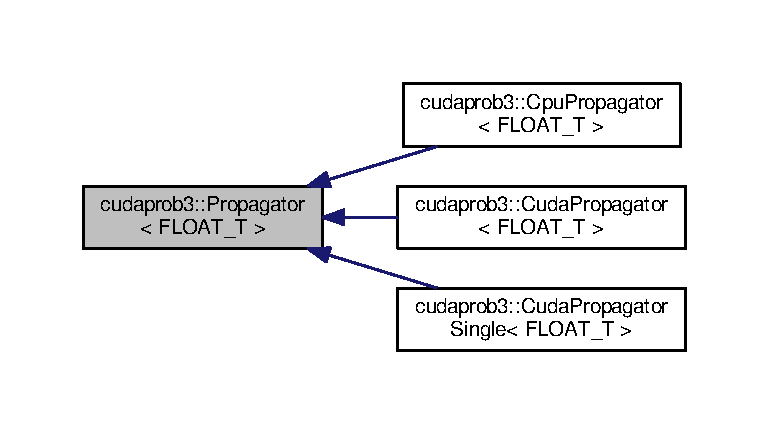
\includegraphics[width=350pt]{classcudaprob3_1_1Propagator__inherit__graph}
\end{center}
\end{figure}
\subsection*{Public Member Functions}
\begin{DoxyCompactItemize}
\item 
\hyperlink{classcudaprob3_1_1Propagator_a460c3f4476cf5d300bdc94574ae175c6}{Propagator} (int n\+\_\+cosines, int n\+\_\+energies)
\begin{DoxyCompactList}\small\item\em Constructor. \end{DoxyCompactList}\item 
\hyperlink{classcudaprob3_1_1Propagator_a22e248af597b6826b49e7ef42057d321}{Propagator} (const \hyperlink{classcudaprob3_1_1Propagator}{Propagator} \&other)
\begin{DoxyCompactList}\small\item\em Copy constructor. \end{DoxyCompactList}\item 
\hyperlink{classcudaprob3_1_1Propagator_a226e189d52e68341b0238d8f50ea7392}{Propagator} (\hyperlink{classcudaprob3_1_1Propagator}{Propagator} \&\&other)
\begin{DoxyCompactList}\small\item\em Move constructor. \end{DoxyCompactList}\item 
\hyperlink{classcudaprob3_1_1Propagator}{Propagator} \& \hyperlink{classcudaprob3_1_1Propagator_aeb44cd674bf25ed8954b6e2d1ff836dc}{operator=} (const \hyperlink{classcudaprob3_1_1Propagator}{Propagator} \&other)
\begin{DoxyCompactList}\small\item\em Copy assignment operator. \end{DoxyCompactList}\item 
\hyperlink{classcudaprob3_1_1Propagator}{Propagator} \& \hyperlink{classcudaprob3_1_1Propagator_a2ca4bda20f63fb8c96b10f2511b8c5f4}{operator=} (\hyperlink{classcudaprob3_1_1Propagator}{Propagator} \&\&other)
\begin{DoxyCompactList}\small\item\em Move assignment operator. \end{DoxyCompactList}\item 
virtual void \hyperlink{classcudaprob3_1_1Propagator_a119a29681c30c9476f0b50ed07cb639d}{set\+Density} (const std\+::vector$<$ F\+L\+O\+A\+T\+\_\+T $>$ \&radii\+\_\+, const std\+::vector$<$ F\+L\+O\+A\+T\+\_\+T $>$ \&rhos\+\_\+)
\begin{DoxyCompactList}\small\item\em Set density information from arrays. \end{DoxyCompactList}\item 
virtual void \hyperlink{classcudaprob3_1_1Propagator_a7d40f7d7e0716e5b532a7a3a228d3b01}{set\+Density\+From\+File} (const std\+::string \&filename)
\begin{DoxyCompactList}\small\item\em Set density information from file. \end{DoxyCompactList}\item 
virtual void \hyperlink{classcudaprob3_1_1Propagator_ad866c252d72ae6cc0ed3fc3b76c7cac7}{set\+M\+N\+S\+Matrix} (F\+L\+O\+A\+T\+\_\+T theta12, F\+L\+O\+A\+T\+\_\+T theta13, F\+L\+O\+A\+T\+\_\+T theta23, F\+L\+O\+A\+T\+\_\+T d\+CP)
\begin{DoxyCompactList}\small\item\em Set mixing angles and cp phase in radians. \end{DoxyCompactList}\item 
virtual void \hyperlink{classcudaprob3_1_1Propagator_adaa3bc796f0bca8ce177f364c559b262}{set\+Neutrino\+Masses} (F\+L\+O\+A\+T\+\_\+T dm12sq, F\+L\+O\+A\+T\+\_\+T dm23sq)
\begin{DoxyCompactList}\small\item\em Set neutrino mass differences (m\+\_\+i\+\_\+j)$^\wedge$2 in (eV)$^\wedge$2. no assumptions about mass hierarchy are made. \end{DoxyCompactList}\item 
virtual void \hyperlink{classcudaprob3_1_1Propagator_a1135d977c5034e982a63c583ab4dad06}{set\+Energy\+List} (const std\+::vector$<$ F\+L\+O\+A\+T\+\_\+T $>$ \&list)
\begin{DoxyCompactList}\small\item\em Set the energy bins. Energies are given in GeV. \end{DoxyCompactList}\item 
virtual void \hyperlink{classcudaprob3_1_1Propagator_ac2beb7d48c566ef0f07666927fbf5e3f}{set\+Cosine\+List} (const std\+::vector$<$ F\+L\+O\+A\+T\+\_\+T $>$ \&list)
\begin{DoxyCompactList}\small\item\em Set cosine bins. Cosines are given in radians. \end{DoxyCompactList}\item 
virtual void \hyperlink{classcudaprob3_1_1Propagator_a5db866f0c9852d65cc2b1e43bbc3bef5}{set\+Production\+Height} (F\+L\+O\+A\+T\+\_\+T height\+KM)
\begin{DoxyCompactList}\small\item\em Set production height in km of neutrinos. \end{DoxyCompactList}\item 
virtual void \hyperlink{classcudaprob3_1_1Propagator_abe3045e287c6a0646474189b3cff14c7}{calculate\+Probabilities} (Neutrino\+Type type)=0
\begin{DoxyCompactList}\small\item\em Calculate the probability of each cell. \end{DoxyCompactList}\item 
virtual F\+L\+O\+A\+T\+\_\+T \hyperlink{classcudaprob3_1_1Propagator_a279ff90463e887754db8379c9582c943}{get\+Probability} (int index\+\_\+cosine, int index\+\_\+energy, Prob\+Type t)=0
\begin{DoxyCompactList}\small\item\em get oscillation weight for specific cosine and energy \end{DoxyCompactList}\end{DoxyCompactItemize}


\subsection{Detailed Description}
\subsubsection*{template$<$class F\+L\+O\+A\+T\+\_\+T$>$\\*
class cudaprob3\+::\+Propagator$<$ F\+L\+O\+A\+T\+\_\+\+T $>$}

Abstract base class of the library which sets up input parameter on the host. Concrete implementation of calcuations is provided in derived classes. 


\begin{DoxyParams}{Parameters}
{\em F\+L\+O\+A\+T\+\_\+T} & The floating point type to use for calculations, i.\+e float, double \\
\hline
\end{DoxyParams}


\subsection{Constructor \& Destructor Documentation}
\index{cudaprob3\+::\+Propagator@{cudaprob3\+::\+Propagator}!Propagator@{Propagator}}
\index{Propagator@{Propagator}!cudaprob3\+::\+Propagator@{cudaprob3\+::\+Propagator}}
\subsubsection[{\texorpdfstring{Propagator(int n\+\_\+cosines, int n\+\_\+energies)}{Propagator(int n_cosines, int n_energies)}}]{\setlength{\rightskip}{0pt plus 5cm}template$<$class F\+L\+O\+A\+T\+\_\+T $>$ {\bf cudaprob3\+::\+Propagator}$<$ F\+L\+O\+A\+T\+\_\+T $>$\+::{\bf Propagator} (
\begin{DoxyParamCaption}
\item[{int}]{n\+\_\+cosines, }
\item[{int}]{n\+\_\+energies}
\end{DoxyParamCaption}
)\hspace{0.3cm}{\ttfamily [inline]}}\hypertarget{classcudaprob3_1_1Propagator_a460c3f4476cf5d300bdc94574ae175c6}{}\label{classcudaprob3_1_1Propagator_a460c3f4476cf5d300bdc94574ae175c6}


Constructor. 


\begin{DoxyParams}{Parameters}
{\em n\+\_\+cosines} & Number cosine bins \\
\hline
{\em n\+\_\+energies} & Number of energy bins \\
\hline
\end{DoxyParams}
\index{cudaprob3\+::\+Propagator@{cudaprob3\+::\+Propagator}!Propagator@{Propagator}}
\index{Propagator@{Propagator}!cudaprob3\+::\+Propagator@{cudaprob3\+::\+Propagator}}
\subsubsection[{\texorpdfstring{Propagator(const Propagator \&other)}{Propagator(const Propagator &other)}}]{\setlength{\rightskip}{0pt plus 5cm}template$<$class F\+L\+O\+A\+T\+\_\+T $>$ {\bf cudaprob3\+::\+Propagator}$<$ F\+L\+O\+A\+T\+\_\+T $>$\+::{\bf Propagator} (
\begin{DoxyParamCaption}
\item[{const {\bf Propagator}$<$ F\+L\+O\+A\+T\+\_\+T $>$ \&}]{other}
\end{DoxyParamCaption}
)\hspace{0.3cm}{\ttfamily [inline]}}\hypertarget{classcudaprob3_1_1Propagator_a22e248af597b6826b49e7ef42057d321}{}\label{classcudaprob3_1_1Propagator_a22e248af597b6826b49e7ef42057d321}


Copy constructor. 


\begin{DoxyParams}{Parameters}
{\em other} & \\
\hline
\end{DoxyParams}
\index{cudaprob3\+::\+Propagator@{cudaprob3\+::\+Propagator}!Propagator@{Propagator}}
\index{Propagator@{Propagator}!cudaprob3\+::\+Propagator@{cudaprob3\+::\+Propagator}}
\subsubsection[{\texorpdfstring{Propagator(\+Propagator \&\&other)}{Propagator(Propagator &&other)}}]{\setlength{\rightskip}{0pt plus 5cm}template$<$class F\+L\+O\+A\+T\+\_\+T $>$ {\bf cudaprob3\+::\+Propagator}$<$ F\+L\+O\+A\+T\+\_\+T $>$\+::{\bf Propagator} (
\begin{DoxyParamCaption}
\item[{{\bf Propagator}$<$ F\+L\+O\+A\+T\+\_\+T $>$ \&\&}]{other}
\end{DoxyParamCaption}
)\hspace{0.3cm}{\ttfamily [inline]}}\hypertarget{classcudaprob3_1_1Propagator_a226e189d52e68341b0238d8f50ea7392}{}\label{classcudaprob3_1_1Propagator_a226e189d52e68341b0238d8f50ea7392}


Move constructor. 


\begin{DoxyParams}{Parameters}
{\em other} & \\
\hline
\end{DoxyParams}


\subsection{Member Function Documentation}
\index{cudaprob3\+::\+Propagator@{cudaprob3\+::\+Propagator}!calculate\+Probabilities@{calculate\+Probabilities}}
\index{calculate\+Probabilities@{calculate\+Probabilities}!cudaprob3\+::\+Propagator@{cudaprob3\+::\+Propagator}}
\subsubsection[{\texorpdfstring{calculate\+Probabilities(\+Neutrino\+Type type)=0}{calculateProbabilities(NeutrinoType type)=0}}]{\setlength{\rightskip}{0pt plus 5cm}template$<$class F\+L\+O\+A\+T\+\_\+T $>$ virtual void {\bf cudaprob3\+::\+Propagator}$<$ F\+L\+O\+A\+T\+\_\+T $>$\+::calculate\+Probabilities (
\begin{DoxyParamCaption}
\item[{Neutrino\+Type}]{type}
\end{DoxyParamCaption}
)\hspace{0.3cm}{\ttfamily [pure virtual]}}\hypertarget{classcudaprob3_1_1Propagator_abe3045e287c6a0646474189b3cff14c7}{}\label{classcudaprob3_1_1Propagator_abe3045e287c6a0646474189b3cff14c7}


Calculate the probability of each cell. 


\begin{DoxyParams}{Parameters}
{\em type} & Neutrino or Antineutrino \\
\hline
\end{DoxyParams}


Implemented in \hyperlink{classcudaprob3_1_1CudaPropagator_abafc49cd41569e985bd3bd9e07b31149}{cudaprob3\+::\+Cuda\+Propagator$<$ F\+L\+O\+A\+T\+\_\+\+T $>$}, \hyperlink{classcudaprob3_1_1CudaPropagatorSingle_a3955e2e44178fd6586cdeec77d597139}{cudaprob3\+::\+Cuda\+Propagator\+Single$<$ F\+L\+O\+A\+T\+\_\+\+T $>$}, and \hyperlink{classcudaprob3_1_1CpuPropagator_adfd6a6c86a5992bce66d0bcf975bc17d}{cudaprob3\+::\+Cpu\+Propagator$<$ F\+L\+O\+A\+T\+\_\+\+T $>$}.

\index{cudaprob3\+::\+Propagator@{cudaprob3\+::\+Propagator}!get\+Probability@{get\+Probability}}
\index{get\+Probability@{get\+Probability}!cudaprob3\+::\+Propagator@{cudaprob3\+::\+Propagator}}
\subsubsection[{\texorpdfstring{get\+Probability(int index\+\_\+cosine, int index\+\_\+energy, Prob\+Type t)=0}{getProbability(int index_cosine, int index_energy, ProbType t)=0}}]{\setlength{\rightskip}{0pt plus 5cm}template$<$class F\+L\+O\+A\+T\+\_\+T $>$ virtual F\+L\+O\+A\+T\+\_\+T {\bf cudaprob3\+::\+Propagator}$<$ F\+L\+O\+A\+T\+\_\+T $>$\+::get\+Probability (
\begin{DoxyParamCaption}
\item[{int}]{index\+\_\+cosine, }
\item[{int}]{index\+\_\+energy, }
\item[{Prob\+Type}]{t}
\end{DoxyParamCaption}
)\hspace{0.3cm}{\ttfamily [pure virtual]}}\hypertarget{classcudaprob3_1_1Propagator_a279ff90463e887754db8379c9582c943}{}\label{classcudaprob3_1_1Propagator_a279ff90463e887754db8379c9582c943}


get oscillation weight for specific cosine and energy 


\begin{DoxyParams}{Parameters}
{\em index\+\_\+cosine} & Cosine bin index (zero based) \\
\hline
{\em index\+\_\+energy} & Energy bin index (zero based) \\
\hline
{\em t} & Specify which probability P(i-\/$>$j) \\
\hline
\end{DoxyParams}


Implemented in \hyperlink{classcudaprob3_1_1CudaPropagator_a3cde10f1ca21db8896420649dc5d4734}{cudaprob3\+::\+Cuda\+Propagator$<$ F\+L\+O\+A\+T\+\_\+\+T $>$}, \hyperlink{classcudaprob3_1_1CudaPropagatorSingle_a7721f79e2e58ab959ba4e295ac8b4b0c}{cudaprob3\+::\+Cuda\+Propagator\+Single$<$ F\+L\+O\+A\+T\+\_\+\+T $>$}, and \hyperlink{classcudaprob3_1_1CpuPropagator_adb5c71e1b00dd5d436f04dfa9db0b364}{cudaprob3\+::\+Cpu\+Propagator$<$ F\+L\+O\+A\+T\+\_\+\+T $>$}.

\index{cudaprob3\+::\+Propagator@{cudaprob3\+::\+Propagator}!operator=@{operator=}}
\index{operator=@{operator=}!cudaprob3\+::\+Propagator@{cudaprob3\+::\+Propagator}}
\subsubsection[{\texorpdfstring{operator=(const Propagator \&other)}{operator=(const Propagator &other)}}]{\setlength{\rightskip}{0pt plus 5cm}template$<$class F\+L\+O\+A\+T\+\_\+T $>$ {\bf Propagator}\& {\bf cudaprob3\+::\+Propagator}$<$ F\+L\+O\+A\+T\+\_\+T $>$\+::operator= (
\begin{DoxyParamCaption}
\item[{const {\bf Propagator}$<$ F\+L\+O\+A\+T\+\_\+T $>$ \&}]{other}
\end{DoxyParamCaption}
)\hspace{0.3cm}{\ttfamily [inline]}}\hypertarget{classcudaprob3_1_1Propagator_aeb44cd674bf25ed8954b6e2d1ff836dc}{}\label{classcudaprob3_1_1Propagator_aeb44cd674bf25ed8954b6e2d1ff836dc}


Copy assignment operator. 


\begin{DoxyParams}{Parameters}
{\em other} & \\
\hline
\end{DoxyParams}
\index{cudaprob3\+::\+Propagator@{cudaprob3\+::\+Propagator}!operator=@{operator=}}
\index{operator=@{operator=}!cudaprob3\+::\+Propagator@{cudaprob3\+::\+Propagator}}
\subsubsection[{\texorpdfstring{operator=(\+Propagator \&\&other)}{operator=(Propagator &&other)}}]{\setlength{\rightskip}{0pt plus 5cm}template$<$class F\+L\+O\+A\+T\+\_\+T $>$ {\bf Propagator}\& {\bf cudaprob3\+::\+Propagator}$<$ F\+L\+O\+A\+T\+\_\+T $>$\+::operator= (
\begin{DoxyParamCaption}
\item[{{\bf Propagator}$<$ F\+L\+O\+A\+T\+\_\+T $>$ \&\&}]{other}
\end{DoxyParamCaption}
)\hspace{0.3cm}{\ttfamily [inline]}}\hypertarget{classcudaprob3_1_1Propagator_a2ca4bda20f63fb8c96b10f2511b8c5f4}{}\label{classcudaprob3_1_1Propagator_a2ca4bda20f63fb8c96b10f2511b8c5f4}


Move assignment operator. 


\begin{DoxyParams}{Parameters}
{\em other} & \\
\hline
\end{DoxyParams}
\index{cudaprob3\+::\+Propagator@{cudaprob3\+::\+Propagator}!set\+Cosine\+List@{set\+Cosine\+List}}
\index{set\+Cosine\+List@{set\+Cosine\+List}!cudaprob3\+::\+Propagator@{cudaprob3\+::\+Propagator}}
\subsubsection[{\texorpdfstring{set\+Cosine\+List(const std\+::vector$<$ F\+L\+O\+A\+T\+\_\+\+T $>$ \&list)}{setCosineList(const std::vector< FLOAT_T > &list)}}]{\setlength{\rightskip}{0pt plus 5cm}template$<$class F\+L\+O\+A\+T\+\_\+T $>$ virtual void {\bf cudaprob3\+::\+Propagator}$<$ F\+L\+O\+A\+T\+\_\+T $>$\+::set\+Cosine\+List (
\begin{DoxyParamCaption}
\item[{const std\+::vector$<$ F\+L\+O\+A\+T\+\_\+T $>$ \&}]{list}
\end{DoxyParamCaption}
)\hspace{0.3cm}{\ttfamily [inline]}, {\ttfamily [virtual]}}\hypertarget{classcudaprob3_1_1Propagator_ac2beb7d48c566ef0f07666927fbf5e3f}{}\label{classcudaprob3_1_1Propagator_ac2beb7d48c566ef0f07666927fbf5e3f}


Set cosine bins. Cosines are given in radians. 


\begin{DoxyParams}{Parameters}
{\em list} & Cosine list \\
\hline
\end{DoxyParams}


Reimplemented in \hyperlink{classcudaprob3_1_1CudaPropagator_afb6f73bd2451d64cfcd2b893b9b86413}{cudaprob3\+::\+Cuda\+Propagator$<$ F\+L\+O\+A\+T\+\_\+\+T $>$}, and \hyperlink{classcudaprob3_1_1CudaPropagatorSingle_ab246f402045676c70d8b9eb5cf8e406d}{cudaprob3\+::\+Cuda\+Propagator\+Single$<$ F\+L\+O\+A\+T\+\_\+\+T $>$}.

\index{cudaprob3\+::\+Propagator@{cudaprob3\+::\+Propagator}!set\+Density@{set\+Density}}
\index{set\+Density@{set\+Density}!cudaprob3\+::\+Propagator@{cudaprob3\+::\+Propagator}}
\subsubsection[{\texorpdfstring{set\+Density(const std\+::vector$<$ F\+L\+O\+A\+T\+\_\+\+T $>$ \&radii\+\_\+, const std\+::vector$<$ F\+L\+O\+A\+T\+\_\+\+T $>$ \&rhos\+\_\+)}{setDensity(const std::vector< FLOAT_T > &radii_, const std::vector< FLOAT_T > &rhos_)}}]{\setlength{\rightskip}{0pt plus 5cm}template$<$class F\+L\+O\+A\+T\+\_\+T $>$ virtual void {\bf cudaprob3\+::\+Propagator}$<$ F\+L\+O\+A\+T\+\_\+T $>$\+::set\+Density (
\begin{DoxyParamCaption}
\item[{const std\+::vector$<$ F\+L\+O\+A\+T\+\_\+T $>$ \&}]{radii\+\_\+, }
\item[{const std\+::vector$<$ F\+L\+O\+A\+T\+\_\+T $>$ \&}]{rhos\+\_\+}
\end{DoxyParamCaption}
)\hspace{0.3cm}{\ttfamily [inline]}, {\ttfamily [virtual]}}\hypertarget{classcudaprob3_1_1Propagator_a119a29681c30c9476f0b50ed07cb639d}{}\label{classcudaprob3_1_1Propagator_a119a29681c30c9476f0b50ed07cb639d}


Set density information from arrays. 

radii\+\_\+ and rhos\+\_\+ must be same size. both radii\+\_\+ and rhos\+\_\+ must be sorted, in the same order. The density (g/cm$^\wedge$3) at a distance (km) from the center of the sphere between radii\+\_\+\mbox{[}i\mbox{]}, exclusive, and radii\+\_\+\mbox{[}j\mbox{]}, inclusive, i $<$ j is assumed to be rhos\+\_\+\mbox{[}j\mbox{]} 
\begin{DoxyParams}{Parameters}
{\em radii\+\_\+} & List of radii \\
\hline
{\em rhos\+\_\+} & List of densities \\
\hline
\end{DoxyParams}


Reimplemented in \hyperlink{classcudaprob3_1_1CudaPropagator_a90deddfaf8ab3c830a60d5ad5fbcfb43}{cudaprob3\+::\+Cuda\+Propagator$<$ F\+L\+O\+A\+T\+\_\+\+T $>$}, and \hyperlink{classcudaprob3_1_1CudaPropagatorSingle_ad2aba9c12a96f429a8ee675c865ceccf}{cudaprob3\+::\+Cuda\+Propagator\+Single$<$ F\+L\+O\+A\+T\+\_\+\+T $>$}.

\index{cudaprob3\+::\+Propagator@{cudaprob3\+::\+Propagator}!set\+Density\+From\+File@{set\+Density\+From\+File}}
\index{set\+Density\+From\+File@{set\+Density\+From\+File}!cudaprob3\+::\+Propagator@{cudaprob3\+::\+Propagator}}
\subsubsection[{\texorpdfstring{set\+Density\+From\+File(const std\+::string \&filename)}{setDensityFromFile(const std::string &filename)}}]{\setlength{\rightskip}{0pt plus 5cm}template$<$class F\+L\+O\+A\+T\+\_\+T $>$ virtual void {\bf cudaprob3\+::\+Propagator}$<$ F\+L\+O\+A\+T\+\_\+T $>$\+::set\+Density\+From\+File (
\begin{DoxyParamCaption}
\item[{const std\+::string \&}]{filename}
\end{DoxyParamCaption}
)\hspace{0.3cm}{\ttfamily [inline]}, {\ttfamily [virtual]}}\hypertarget{classcudaprob3_1_1Propagator_a7d40f7d7e0716e5b532a7a3a228d3b01}{}\label{classcudaprob3_1_1Propagator_a7d40f7d7e0716e5b532a7a3a228d3b01}


Set density information from file. 

File must contain two columns where the first column contains the radius (km) and the second column contains the density (g/cm³). The first row must have the radius 0. The last row must have to radius of the sphere


\begin{DoxyParams}{Parameters}
{\em filename} & File with density information \\
\hline
\end{DoxyParams}


Reimplemented in \hyperlink{classcudaprob3_1_1CudaPropagator_a61124bdc43a631b55ad1e9bd36a872eb}{cudaprob3\+::\+Cuda\+Propagator$<$ F\+L\+O\+A\+T\+\_\+\+T $>$}.

\index{cudaprob3\+::\+Propagator@{cudaprob3\+::\+Propagator}!set\+Energy\+List@{set\+Energy\+List}}
\index{set\+Energy\+List@{set\+Energy\+List}!cudaprob3\+::\+Propagator@{cudaprob3\+::\+Propagator}}
\subsubsection[{\texorpdfstring{set\+Energy\+List(const std\+::vector$<$ F\+L\+O\+A\+T\+\_\+\+T $>$ \&list)}{setEnergyList(const std::vector< FLOAT_T > &list)}}]{\setlength{\rightskip}{0pt plus 5cm}template$<$class F\+L\+O\+A\+T\+\_\+T $>$ virtual void {\bf cudaprob3\+::\+Propagator}$<$ F\+L\+O\+A\+T\+\_\+T $>$\+::set\+Energy\+List (
\begin{DoxyParamCaption}
\item[{const std\+::vector$<$ F\+L\+O\+A\+T\+\_\+T $>$ \&}]{list}
\end{DoxyParamCaption}
)\hspace{0.3cm}{\ttfamily [inline]}, {\ttfamily [virtual]}}\hypertarget{classcudaprob3_1_1Propagator_a1135d977c5034e982a63c583ab4dad06}{}\label{classcudaprob3_1_1Propagator_a1135d977c5034e982a63c583ab4dad06}


Set the energy bins. Energies are given in GeV. 


\begin{DoxyParams}{Parameters}
{\em list} & Energy list \\
\hline
\end{DoxyParams}


Reimplemented in \hyperlink{classcudaprob3_1_1CudaPropagator_aa2fd3a1c4c30ea967e5ac14a32ee5b7f}{cudaprob3\+::\+Cuda\+Propagator$<$ F\+L\+O\+A\+T\+\_\+\+T $>$}, and \hyperlink{classcudaprob3_1_1CudaPropagatorSingle_a0f31f396035587744335cc6907124066}{cudaprob3\+::\+Cuda\+Propagator\+Single$<$ F\+L\+O\+A\+T\+\_\+\+T $>$}.

\index{cudaprob3\+::\+Propagator@{cudaprob3\+::\+Propagator}!set\+M\+N\+S\+Matrix@{set\+M\+N\+S\+Matrix}}
\index{set\+M\+N\+S\+Matrix@{set\+M\+N\+S\+Matrix}!cudaprob3\+::\+Propagator@{cudaprob3\+::\+Propagator}}
\subsubsection[{\texorpdfstring{set\+M\+N\+S\+Matrix(\+F\+L\+O\+A\+T\+\_\+\+T theta12, F\+L\+O\+A\+T\+\_\+\+T theta13, F\+L\+O\+A\+T\+\_\+\+T theta23, F\+L\+O\+A\+T\+\_\+\+T d\+C\+P)}{setMNSMatrix(FLOAT_T theta12, FLOAT_T theta13, FLOAT_T theta23, FLOAT_T dCP)}}]{\setlength{\rightskip}{0pt plus 5cm}template$<$class F\+L\+O\+A\+T\+\_\+T $>$ virtual void {\bf cudaprob3\+::\+Propagator}$<$ F\+L\+O\+A\+T\+\_\+T $>$\+::set\+M\+N\+S\+Matrix (
\begin{DoxyParamCaption}
\item[{F\+L\+O\+A\+T\+\_\+T}]{theta12, }
\item[{F\+L\+O\+A\+T\+\_\+T}]{theta13, }
\item[{F\+L\+O\+A\+T\+\_\+T}]{theta23, }
\item[{F\+L\+O\+A\+T\+\_\+T}]{d\+CP}
\end{DoxyParamCaption}
)\hspace{0.3cm}{\ttfamily [inline]}, {\ttfamily [virtual]}}\hypertarget{classcudaprob3_1_1Propagator_ad866c252d72ae6cc0ed3fc3b76c7cac7}{}\label{classcudaprob3_1_1Propagator_ad866c252d72ae6cc0ed3fc3b76c7cac7}


Set mixing angles and cp phase in radians. 


\begin{DoxyParams}{Parameters}
{\em theta12} & \\
\hline
{\em theta13} & \\
\hline
{\em theta23} & \\
\hline
{\em d\+CP} & \\
\hline
\end{DoxyParams}


Reimplemented in \hyperlink{classcudaprob3_1_1CudaPropagator_ad4fd47cd63e3b45919ae80d876698ac4}{cudaprob3\+::\+Cuda\+Propagator$<$ F\+L\+O\+A\+T\+\_\+\+T $>$}.

\index{cudaprob3\+::\+Propagator@{cudaprob3\+::\+Propagator}!set\+Neutrino\+Masses@{set\+Neutrino\+Masses}}
\index{set\+Neutrino\+Masses@{set\+Neutrino\+Masses}!cudaprob3\+::\+Propagator@{cudaprob3\+::\+Propagator}}
\subsubsection[{\texorpdfstring{set\+Neutrino\+Masses(\+F\+L\+O\+A\+T\+\_\+\+T dm12sq, F\+L\+O\+A\+T\+\_\+\+T dm23sq)}{setNeutrinoMasses(FLOAT_T dm12sq, FLOAT_T dm23sq)}}]{\setlength{\rightskip}{0pt plus 5cm}template$<$class F\+L\+O\+A\+T\+\_\+T $>$ virtual void {\bf cudaprob3\+::\+Propagator}$<$ F\+L\+O\+A\+T\+\_\+T $>$\+::set\+Neutrino\+Masses (
\begin{DoxyParamCaption}
\item[{F\+L\+O\+A\+T\+\_\+T}]{dm12sq, }
\item[{F\+L\+O\+A\+T\+\_\+T}]{dm23sq}
\end{DoxyParamCaption}
)\hspace{0.3cm}{\ttfamily [inline]}, {\ttfamily [virtual]}}\hypertarget{classcudaprob3_1_1Propagator_adaa3bc796f0bca8ce177f364c559b262}{}\label{classcudaprob3_1_1Propagator_adaa3bc796f0bca8ce177f364c559b262}


Set neutrino mass differences (m\+\_\+i\+\_\+j)$^\wedge$2 in (eV)$^\wedge$2. no assumptions about mass hierarchy are made. 


\begin{DoxyParams}{Parameters}
{\em dm12sq} & \\
\hline
{\em dm23sq} & \\
\hline
\end{DoxyParams}


Reimplemented in \hyperlink{classcudaprob3_1_1CudaPropagator_abb9d8cc79c88f9cf6886cd334ed9e869}{cudaprob3\+::\+Cuda\+Propagator$<$ F\+L\+O\+A\+T\+\_\+\+T $>$}.

\index{cudaprob3\+::\+Propagator@{cudaprob3\+::\+Propagator}!set\+Production\+Height@{set\+Production\+Height}}
\index{set\+Production\+Height@{set\+Production\+Height}!cudaprob3\+::\+Propagator@{cudaprob3\+::\+Propagator}}
\subsubsection[{\texorpdfstring{set\+Production\+Height(\+F\+L\+O\+A\+T\+\_\+\+T height\+K\+M)}{setProductionHeight(FLOAT_T heightKM)}}]{\setlength{\rightskip}{0pt plus 5cm}template$<$class F\+L\+O\+A\+T\+\_\+T $>$ virtual void {\bf cudaprob3\+::\+Propagator}$<$ F\+L\+O\+A\+T\+\_\+T $>$\+::set\+Production\+Height (
\begin{DoxyParamCaption}
\item[{F\+L\+O\+A\+T\+\_\+T}]{height\+KM}
\end{DoxyParamCaption}
)\hspace{0.3cm}{\ttfamily [inline]}, {\ttfamily [virtual]}}\hypertarget{classcudaprob3_1_1Propagator_a5db866f0c9852d65cc2b1e43bbc3bef5}{}\label{classcudaprob3_1_1Propagator_a5db866f0c9852d65cc2b1e43bbc3bef5}


Set production height in km of neutrinos. 

Adds a layer of length height\+KM with zero density to the density model 
\begin{DoxyParams}{Parameters}
{\em height\+KM} & Set neutrino production height \\
\hline
\end{DoxyParams}


Reimplemented in \hyperlink{classcudaprob3_1_1CudaPropagator_ad639f2aa32a548b74a9a9c82d498b24a}{cudaprob3\+::\+Cuda\+Propagator$<$ F\+L\+O\+A\+T\+\_\+\+T $>$}.



The documentation for this class was generated from the following file\+:\begin{DoxyCompactItemize}
\item 
propagator.\+hpp\end{DoxyCompactItemize}

%--- End generated contents ---

% Index
\backmatter
\newpage
\phantomsection
\clearemptydoublepage
\addcontentsline{toc}{chapter}{Index}
\printindex

\end{document}
